%!TEX program = xelatex
% 使用 ctexart 文类,UTF-8 编码
\documentclass[UTF8]{ctexart}
\usepackage{cite}
\usepackage{geometry}
\usepackage{graphicx}
\usepackage[colorlinks,
            linkcolor=red,
            anchorcolor=blue,
            citecolor=green
            ]{hyperref}
\geometry{a4paper,scale=0.8}
\usepackage{indentfirst}
\setlength{\parindent}{2em}
\usepackage{ listings} 
\usepackage{ xcolor} 
\usepackage{fontspec}
\setmonofont{Consolas}

\begin{document}
面试问题总结
\begin{abstract}
    在开发面试中,会遇到各种各样的问题,这里我们对面试中遇到的问题进行总结,方便自己经常性的反思和理解一些算法和常见的问题。帮助后续的程序面试的复习。
\end{abstract}

\section{魔鬼问题}
\subsection{题目}
现在有10个人被一个魔鬼逮住了。魔鬼对于直接把人杀掉的方法不感兴趣了。于是,他就想了一个杀人的新花样。
是这样的,一天晚上,魔鬼向这十个人宣布了游戏规则 ,即明早他要把他们10个人排成一排,然后从一堆既有无限多的
白帽子混会着无限多的黑帽子的帽子堆里为每个人随机抽取一顶帽子,给他们10个人都戴上帽子。因为 10个人是排成一
排的,所以排在第10个的人可以看到前面9个人帽子的颜色,排在第9个人可以看到前面8个人的帽子的颜色,...以此类推。然后,魔鬼会从排在 第10个人开始,问他,你头上的帽子的颜色是白色还是黑色,如果答对了,就放他走;如果答错了,
就被杀掉。然后同样问排在第9位的人,然后问同样问排在第8位的 人,...以此类推。在这其中,10个人所能做的只有当他
被魔鬼问到的时候,答白色或者黑色。不能有超越此范围的任何行动,不然,魔鬼会把他们10个人全都杀死 。 现在,魔鬼
给他们10个人一个晚上的时间去商量一个对策,使得他们中能存活下来的人越多越好。请问,你会有什么样的对策,请计
算出按照你的对策执行时最坏的情况 下,他们中能有多少人能100\%够活下来?期望能活下来的人数又是多少?
\subsection{思路}
 让答的人给前面的人足够多的信息
 \subsection{解答}
从只能回答白或黑,也就是只能2中选1,从而联想到二进制和奇偶性。二进制一下子没想出什么好方法,奇偶性有一些提
示,所以从奇偶性入手。第10个人 以他所见到的9个帽子中白帽的数量的奇偶性作答,例如大家约定白代表偶,黑代表奇,
则第10个人的回答是前9个帽子中白帽的数量的奇偶。他自己有50%的机会。 第9个人听到他的回答后,结合他看到的8顶帽
子中白帽的奇偶,可以知道自己的帽子的颜色,如实作答。第8个人知道9顶帽子中白帽的奇偶,加上听到第9顶帽子的颜 
色,就可以知道前8顶帽子中白帽的奇偶(如果第9个人答白,则前8顶中的白帽奇偶性与第第10个人所说的相反;如果第9
个人答黑,则相同),再结合所看到前7顶 帽子中的白帽数量,也可以推出自己的帽子颜色,也如实作答。依此类推
,前9个人都可以活下来,第10个人有一半机会。
\section{Top K问题}
\subsection{问题}
给一个超过100G大小的log file, log中存着IP地址, 设计算法找到出现次数最多的IP地址?
与上题条件相同,如何找到top K的IP?如何直接用Linux系统命令实现?
\subsection{解答}
Hash分桶法: 
• 将100G文件分成1000份,将每个IP地址映射到相应文件中:$file_id = hash(ip) \% 1000 $
• 在每个文件中分别求出最高频的IP,再合并 Hash分桶法: 
• 使用Hash分桶法把数据分发到不同文件 
• 各个文件分别统计top K 
• 最后Top K汇总 
Linux命令,假设$top 10:sort log_file | uniq -c | sort -nr k1,1 | head -10$
\section{http和https的区别}
\subsection{Http和Https的基本概念}

Http:超文本传输协议(Http,HyperText Transfer Protocol)是互联网上应用最为广泛的一种网络协议。
设计Http最初的目的是为了提供一种发布和接收HTML页面的方法。它可以使浏览器更加高效。Http协议是以明文
方式发送信息的,如果黑客截取了Web浏览器和服务器之间的传输报文,就可以直接获得其中的信息。

Https:是以安全为目标的Http通道,是Http的安全版。Https的安全基础是SSL。SSL协议位于TCP/IP协议与各
种应用层协议之间,为数据通讯提供安全支持。SSL协议可分为两层:SSL记录协议(SSL Record Protocol),它
建立在可靠的传输协议(如TCP)之上,为高层协议提供数据封装、压缩、加密等基本功能的支持。SSL握手协议(SSL 
Handshake Protocol),它建立在SSL记录协议之上,用于在实际的数据传输开始前,通讯双方进行身份认证、协商
加密算法、交换加密密钥等。
\subsection{Http与Https的区别}
1、https协议需要到CA申请证书,一般免费证书较少,因而需要一定费用。(原来网易官网是http,而网易邮箱
	是https。)

2、http是超文本传输协议,信息是明文传输,https则是具有安全性的ssl加密传输协议。

3、http和https使用的是完全不同的连接方式,用的端口也不一样,前者是80,后者是443。

4、http的连接很简单,是无状态的。Https协议是由SSL+Http协议构建的可进行加密传输、身份认证的网络协议,
比http协议安全。(无状态的意思是其数据包的发送、传输和接收都是相互独立的。无连接的意思是指通信双方都不
	长久的维持对方的任何信息。)
\subsection{Https的优点}
1、使用Https协议可认证用户和服务器,确保数据发送到正确的客户机和服务器。

2、Https协议是由SSL+Http协议构建的可进行加密传输、身份认证的网络协议,要比http协议安全,可防止数据在
传输过程中不被窃取、修改,确保数据的完整性。

3、Https是现行架构下最安全的解决方案,虽然不是绝对安全,但它大幅增加了中间人攻击的成本。
\subsection{Https的缺点(对比优点)}
1、Https协议握手阶段比较费时,会使页面的加载时间延长近。

2、Https连接缓存不如Http高效,会增加数据开销,甚至已有的安全措施也会因此而受到影响;

3、SSL证书通常需要绑定IP,不能在同一IP上绑定多个域名,IPv4资源不可能支撑这个消耗。

4、Https协议的加密范围也比较有限。最关键的,SSL证书的信用链体系并不安全,特别是在某些国家可以控制CA根
证书的情况下,中间人攻击一样可行。
\subsection{Https的连接过程}
\begin{figure}[htbp]
\centering
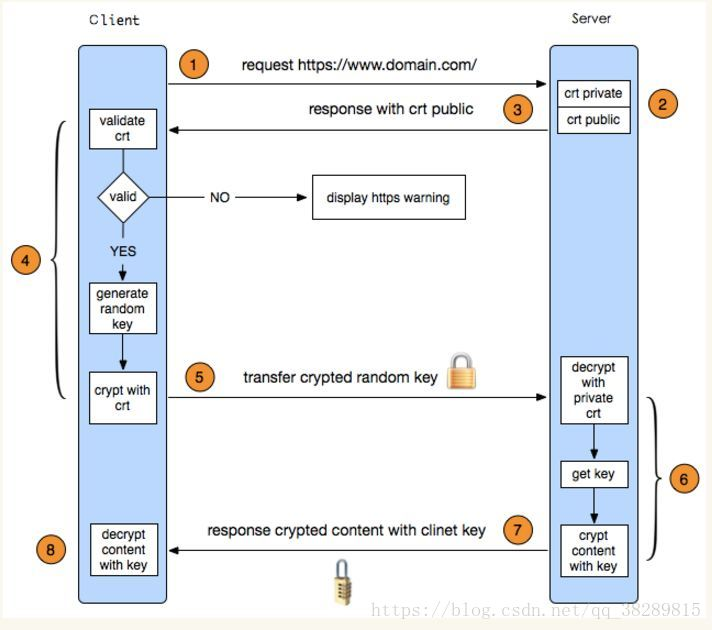
\includegraphics[height=6.0cm,width=9.5cm]{Figure/20180709141944471.jpg}
\caption{Https的连接过程}
\end{figure}
图片中的过程是按8个步骤分的,但是网上有更详细的步骤,所以我把详细的过程和这个图片配在一起。

①客户端的浏览器向服务器发送请求,并传送客户端SSL 协议的版本号,加密算法的种类,产生的随机数,以及其他
服务器和客户端之间通讯所需要的各种信息。

②服务器向客户端传送SSL 协议的版本号,加密算法的种类,随机数以及其他相关信息,同时服务器还将向客户端传
送自己的证书。

③客户端利用服务器传过来的信息验证服务器的合法性,服务器的合法性包括:证书是否过期,发行服务器证书的CA
 是否可靠,发行者证书的公钥能否正确解开服务器证书的“发行者的数字签名”,服务器证书上的域名是否和服务器
 的实际域名相匹配。如果合法性验证没有通过,通讯将断开;如果合法性验证通过,将继续进行第四步。

④用户端随机产生一个用于通讯的“对称密码”,然后用服务器的公钥(服务器的公钥从步骤②中的服务器的证书中获得)
对其加密,然后将加密后的“预主密码”传给服务器。

⑤如果服务器要求客户的身份认证(在握手过程中为可选),用户可以建立一个随机数然后对其进行数据签名,将这个
含有签名的随机数和客户自己的证书以及加密过的“预主密码”一起传给服务器。

⑥如果服务器要求客户的身份认证,服务器必须检验客户证书和签名随机数的合法性,具体的合法性验证过程包括:客
户的证书使用日期是否有效,为客户提供证书的CA 是否可靠,发行CA 的公钥能否正确解开客户证书的发行CA 的数字
签名,检查客户的证书是否在证书废止列表(CRL)中。检验如果没有通过,通讯立刻中断;如果验证通过,服务器将用
自己的私钥解开加密的“预主密码”,然后执行一系列步骤来产生主通讯密码(客户端也将通过同样的方法产生相同的主
通讯密码)。

⑦服务器和客户端用相同的主密码即“通话密码”,一个对称密钥用于SSL 协议的安全数据通讯的加解密通讯。同时在SSL
通讯过程中还要完成数据通讯的完整性,防止数据通讯中的任何变化。

⑧客户端向服务器端发出信息,指明后面的数据通讯将使用的步骤⑦中的主密码为对称密钥,同时通知服务器客户端的握
手过程结束。

⑨服务器向客户端发出信息,指明后面的数据通讯将使用的步骤⑦中的主密码为对称密钥,同时通知客户端服务器端的握
手过程结束。

⑩SSL 的握手部分结束,SSL 安全通道的数据通讯开始,客户和服务器开始使用相同的对称密钥进行数据通讯,同时进行
通讯完整性的检验。


\section{Java面试的问题}
下面是汇总的校招Java后台开发面试考点
\begin{figure}[htbp]
\centering
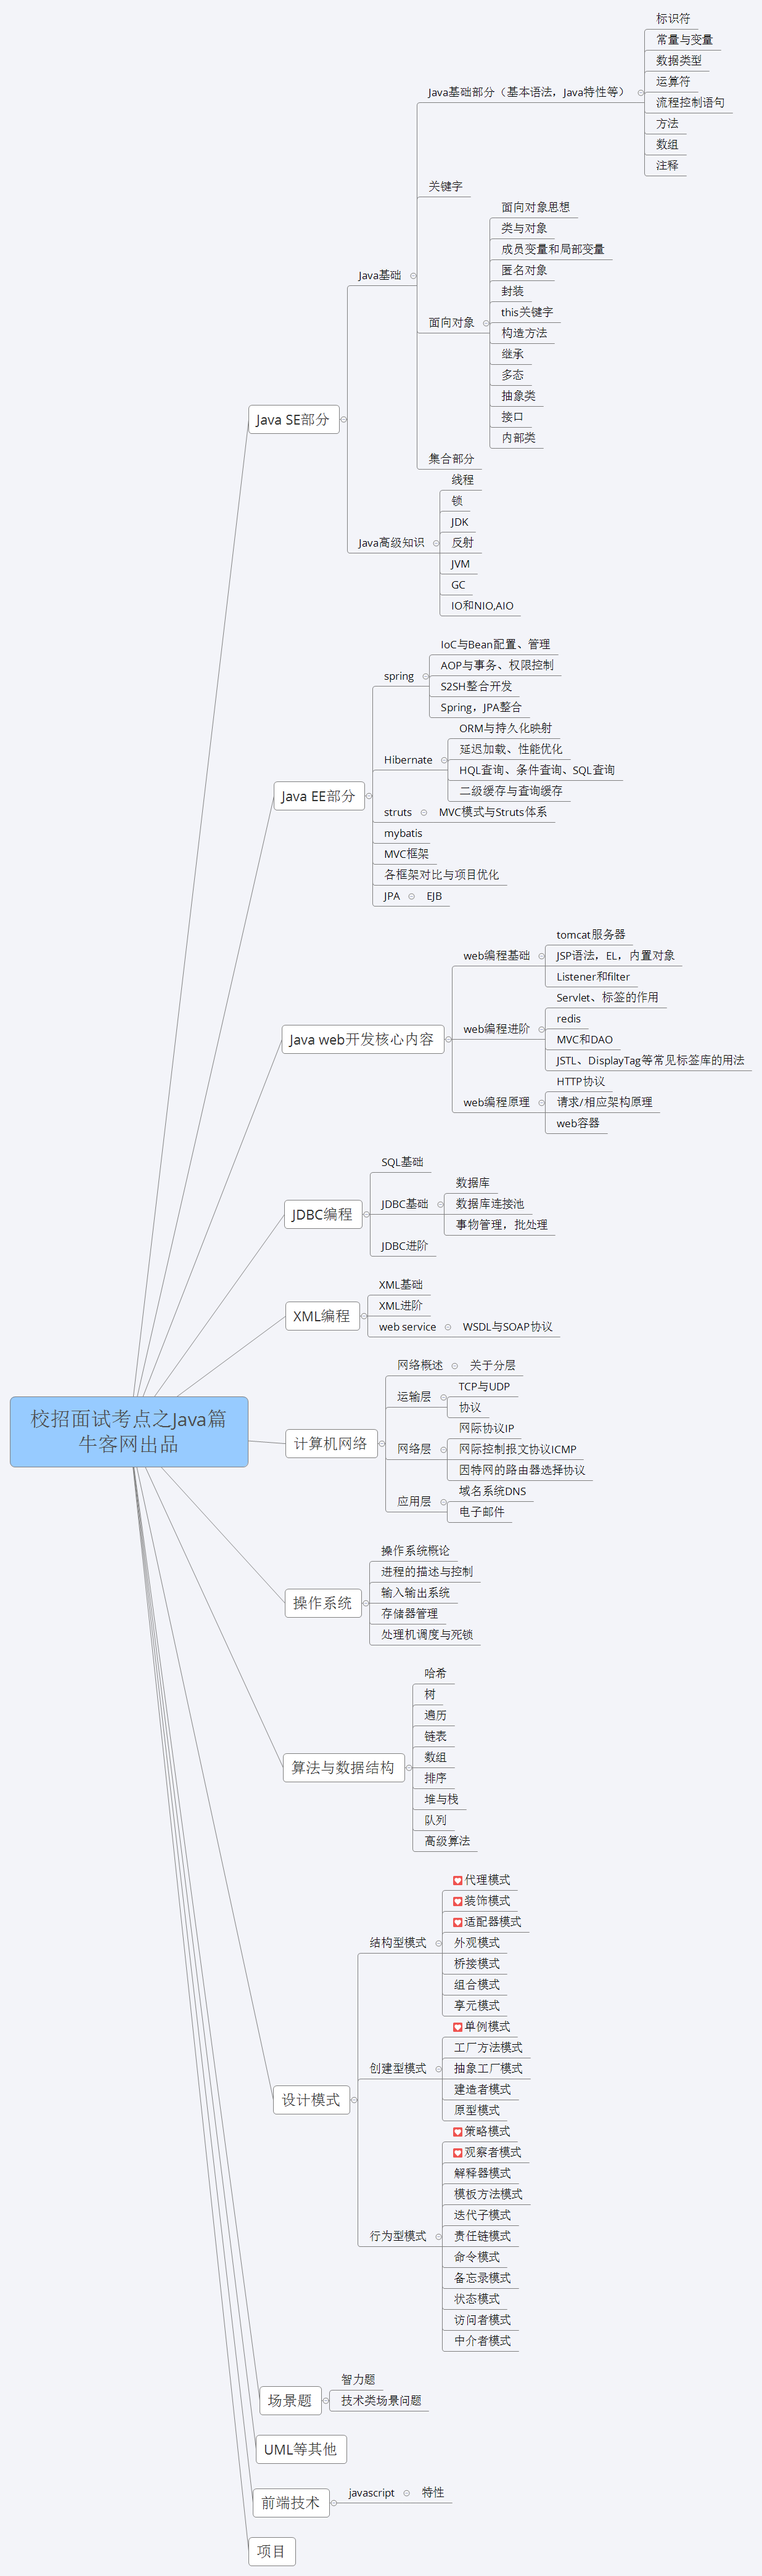
\includegraphics[height=1\linewidth,width=1\textwidth]{Figure/Java.png}
\caption{Java校招面试考点}
\end{figure}

\section{后台开发面试}

\subsubsection{1.自我介绍}
自我介绍主要是对自己的一些简单的情况进行介绍,这部分的主要工作是自己的学习经历,包括在学校发表的论文等。
\subsubsection{2.项目介绍}
需要对自己的项目足够熟悉,每个技术栈知识点非常熟悉,写在简历里面的项目每一个技术栈知识点都要足够熟悉原理用法和一些注意事项

\subsubsection{3.接口和抽象类的区别}
1.抽象类:如果一个类中包含了抽象方法,那么这个类就是抽象类.在Java中可以通过把某些方法声明abstract(abstract只能用来修饰类或者方法不能用来修饰属性)来表示一个类是抽象类。

2.接口就是一个方法的集合,接口中所有的方法都是没有方法体的,通过关键字interface来实现

相同点:
1)都不能被实例化

2)接口的实现类或者抽象类的子类都只有实现了接口或抽象类中的方法后才能被实例化

不同点:
1.在Java8之前接口只有定义,其方法不能在接口中实现(Java8 之后接口方法可以有默认实现),只有实现接口的类才能实现接口中定义的方法。抽象类可以定义和实现,即其方法可以在抽象类中实现 。抽象类可以有非抽象方法

2.一个类可以实现(implements)多个接口,但是最多只能实现(extends)一个抽象类。因此接口可以间接的达到多重继承的目的

3.接口强调的是特定功能的实现,设计理念是一种"has - a"的关系,而抽象类强调的所属关系,其设计理念是"is - a"的关系(ps: has -a 这种事物(羊毛)属于那种事物的一部分(绵羊)! is - a 这种事物(绵羊)属于那种事物(羊)的一个种类)

4.接口中的成员(实例)变量默认为public static final 只能够有静态的不能被修改的数据成员,而且必须给其赋初值,接口中的方法只能用public 和 abstract修饰.但是抽象类不一定

接口是一种特殊形式的抽象类,使用接口完全有可能实现与抽象类相同的操做.通常接口用于比实现比较常用的功能,便于日后维护或者添加删除方法;而抽象类更倾向于充当公共类的角色,不适用于日后重新对里面的代码进行修改.此外接口可以继承接口,抽象类可以实现接口,抽象类也可以继承具体的类,抽象类中可以有静态的main方法

\subsubsection{4.多态}
多态表示当同一个操作作用在不同对象时,会有不同的语义,从而产生不同的结果。3+4和“3”+“4”

Java的多态性可以概括成"一个接口,两种方法"分为两种编译时的多态和运行时的多态。编译时的多态主要是指方法的重载(overload),运行时的多态主要是指方法的覆盖(override),接口也是运行时的多态

运行时的多态的三种情况:

1、父类有方法,子类有覆盖方法:编译通过,执行子类方法。

2、父类有方法,子类没覆盖方法:编译通过,执行父类方法(子类继承)。

3、父类没方法,子类有方法:编译失败,无法执行。

==方法带final、static、private时是编译时多态,因为可以直接确定调用哪个方法。==

\subsubsection{5.重载和覆盖}
重载:发生在一个类中,方法名必须相同,参数类型不同,个数不同,顺序不同,方法返回值和访问修饰符可以不同,发生在编译时

重写:发生在父子类中,方法名,参数列表必须相同,返回值必须小于等于父类,抛出异常的范围必须小于等于父类,访问修饰符范围必须大于等于父类,父类为private则不能重写

函数时不能以返回值来区分的,返回值时函数运行之后的一个状态。保持调用这与被调用这之间的通信

\subsubsection{6.spring}
1.动态代理
代理类在程序运行时创建的代理方式被称为动态代理。代理类并不是在Java代码中定义的,而是在运行时根据我们在Java代码中的“指示”动态生成的。方法实现前后加入对应的公共功能

基于接口
jdk的动态代理时基于Java 的反射机制来实现的,是Java 原生的一种代理方式。他的实现原理就是让代理类和被代理类实现同一接口,代理类持有目标对象来达到方法拦截的作用。通过接口的方式有两个弊端一个就是必须保证被代理类有接口,另一个就是如果相对被代理类的方法进行代理拦截,那么就要保证这些方法都要在接口中声明。接口继承的是java.lang.reflect.InvocationHandler;

基于继承
cglib动态代理使用的ASM这个非常强大的Java字节码生成框架来生成class ,比jdk动态代理ide效率高。基于继承的实现动态代理,可以直接通过super关键字来调用被代理类的方法.子类可以调用父类的方法

2.AOP
面向切面编程。(Aspect-Oriented Programming) 。AOP可以说是对OOP的补充和完善。OOP引入封装、 继承和多态性等概念来建立一种对象层次结构,用以模拟公共行为的一个集合。实现AOP的技术,主要分为两大类: 一是采用动态代理技术,利用截取消息的方式,对该消息进行装饰,以取代原有对象行为的执行;二是采用静态织入 的方式,引入特定的语法创建“方面”,从而使得编译器可以在编译期间织入有关“方面”的代码,属于静态代理。

1.面向切面编程提供声明式事务管理
2.spring支持用户自定义的切面

面向切面编程(aop)是对面向对象编程(oop)的补充, 面向对象编程将程序分解成各个层次的对象,面向切面编程将程序运行过程分解成各个切面。 AOP从程序运行角度考虑程序的结构,提取业务处理过程的切面,oop是静态的抽象,aop是动态的抽象, 是对应用执行过程中的步骤进行抽象,,从而获得步骤之间的逻辑划分。

aop框架具有的两个特征:
1.各个步骤之间的良好隔离性
2.源代码无关性

2.1AOP
springAOP 的具体加载步骤:

1、当 spring 容器启动的时候,加载了 spring 的配置文件

2、为配置文件中的所有 bean 创建对象

3、spring 容器会解析 aop:config 的配置

 1、解析切入点表达式,用切入点表达式和纳入 spring 容器中的 bean 做匹配.如果匹配成功,则会为该 bean 创建代理对象,代理对象的方法=目标方法+通知 如果匹配不成功,不会创建代理对象

4、在客户端利用 context.getBean() 获取对象时,如果该对象有代理对象,则返回代理对象;如果没有,则返回目标对象

说明:如果目标类没有实现接口,则 spring 容器会采用 cglib 的方式产生代理对象,如果实现了接口,则会采用 jdk 的方式

3.IOC
控制反转也叫依赖注入。IOC利用java反射机制,AOP利用代理模式。IOC 概念看似很抽象,但是很容易理解。 说简单点就是将对象交给容器管理,你只需要在spring配置文件中配置对应的bean以及设置相关的属性,让spring 容器来生成类的实例对象以及管理对象。在spring容器启动的时候,spring会把你在配置文件中配置的bean都初始 化好,然后在你需要调用的时候,就把它已经初始化好的那些bean分配给你需要调用这些bean的类

XML–—读取––-> resoure----解析------->BeanDefinition––—注入––––->BeanFactory

详细解析

依赖注入(Dependecy Injection)和控制反转(Inversion of Control)是同一个概念,具体的讲:当某个角色需要另外一个角色协助的时候,在传统的程序设计过程中,通常由调用者来创建被调用者的实例。但在spring中创建被调用者的工作不再由调用者来完成,因此称为控制反转。创建被调用者的工作由spring来完成,然后注入调用者
因此也称为依赖注入。
spring以动态灵活的方式来管理对象 , 注入的两种方式,设置注入和构造注入。
设置注入的优点:直观,自然
构造注入的优点:可以在构造器中决定依赖关系的顺序。

Bean的生命周期

可以简述为以下九步

实例化bean对象(通过构造方法或者工厂方法)
设置对象属性(setter等)(依赖注入)
如果Bean实现了BeanNameAware接口,工厂调用Bean的setBeanName()方法传递Bean的ID。(和下面的一条均属于检查Aware接口)
如果Bean实现了BeanFactoryAware接口,工厂调用setBeanFactory()方法传入工厂自身
将Bean实例传递给Bean的前置处理器的postProcessBeforeInitialization(Object bean, String beanname)方法
调用Bean的初始化方法
将Bean实例传递给Bean的后置处理器的postProcessAfterInitialization(Object bean, String beanname)方法
使用Bean容器关闭之前,调用Bean的销毁方法


4.spring 中Bean的单例和多例模式的使用条件

spring生成的对象默认都是单例(singleton)的.可以通过scope改成多例. 对象在整个系统中只有一份,所有的请求都用一个对象来处理,如service和dao层的对象一般是单例的。

为什么使用单例:因为没有必要每个请求都新建一个对象的时候,因为这样会浪费CPU和内存。

prototype 多例模式:对象在整个系统中可以有多个实例,每个请求用一个新的对象来处理,如action。

为什么使用多例:防止并发问题;即一个请求改变了对象的状态,此时对象又处理另一个请求,而之前请求对对象的状态改变导致了对象对另一个请求做了错误的处理;

5.SSM(顺丰)
5.1SSM各层关系
5.2 为什么注入的是接口(接口多继承)
5.3 Spring的优点
1.降低了组件之间的耦合性 ,实现了软件各层之间的解耦
2.可以使用容易提供的众多服务,如事务管理,消息服务等
3.容器提供单例模式支持
4.容器提供了AOP技术,利用它很容易实现如权限拦截,运行期监控等功能
5.容器提供了众多的辅助类,能加快应用的开发
6.spring对于主流的应用框架提供了集成支持,如hibernate,JPA,Struts等
7.spring属于低侵入式设计,代码的污染极低
8.独立于各种应用服务器
9.spring的DI机制降低了业务对象替换的复杂性
10.Spring的高度开放性,并不强制应用完全依赖于Spring,开发者可以自由选择spring的部分或全部
Spring MVC 的处理过程
(1)客户端通过url发送请求
(2-3)核心控制器Dispatcher Servlet接收到请求,通过系统或自定义的映射器配置找到对应的handler,并将url映射的控制器controller返回给核心控制器。
(4)通过核心控制器找到系统或默认的适配器
(5-7)由找到的适配器,调用实现对应接口的处理器,并将结果返回给适配器,结果中包含数据模型和视图对象,再由适配器返回给核心控制器
(8-9)核心控制器将获取的数据和视图结合的对象传递给视图解析器,获取解析得到的结果,并由视图解析器响应给核心控制器
(10)核心控制器将结果返回给客户端
\subsubsection{7.数据库}
7.1 数据库的三范式以及内外连接
1.数据库的三范式
第一范式(1NF):
指的是数据库表的中的每一列都是不可分割的基本数据项,同一列中不能有多个值。第一范式要求属性值是不可再分割成的更小的部分。第一范式简而言之就是强调的是列的原子性,即列不能够再分成其他几列。例如有一个列是电话号码一个人可能有一个办公电话一个移动电话。第一范式就需要拆开成两个属性。

第二范式(2NF):
第二范式首先是第一范式,同时还需要包含两个方面的内容,一是表必须要有一个主键;二是没有包含主键中的列必须完全依赖主键,而不能只是依赖于主键的一部分。

例如在一个订单中可以订购多种产品,所以单单一个 OrderID 是不足以成为主键的,主键应该是(OrderID,ProductID)。显而易见 Discount(折扣),Quantity(数量)完全依赖(取决)于主键(OderID,ProductID),而 UnitPrice,ProductName 只依赖于 ProductID。所以 OrderDetail 表不符合 2NF。不符合 2NF 的设计容易产生冗余数据。 可以把【OrderDetail】表拆分为【OrderDetail】(OrderID,ProductID,Discount,Quantity)和【Product】(ProductID,UnitPrice,ProductName)来消除原订单表中UnitPrice,ProductName多次重复的情况。

第三范式(3NF):

首先是第二范式,例外非主键列必须依赖于主键,不能存在传递。也就是说不能存在非主键列A依赖于非主键列B,然后B依赖于主键列

考虑一个订单表【Order】(OrderID,OrderDate,CustomerID,CustomerName,CustomerAddr,CustomerCity)主键是(OrderID)。
其中 OrderDate,CustomerID,CustomerName,CustomerAddr,CustomerCity 等非主键列都完全依赖于主键(OrderID),所以符合 2NF。不过问题是 CustomerName,CustomerAddr,CustomerCity 直接依赖的是 CustomerID(非主键列),而不是直接依赖于主键,它是通过传递才依赖于主键,所以不符合 3NF。

通过拆分【Order】为【Order】(OrderID,OrderDate,CustomerID)和【Customer】(CustomerID,CustomerName,CustomerAddr,CustomerCity)从而达到 3NF。

==二范式(2NF)和第三范式(3NF)的概念很容易混淆,区分它们的关键点在于,2NF:非主键列是否完全依赖于主键,还是依赖于主键的一部分;3NF:非主键列是直接依赖于主键,还是直接依赖于非主键列。==

2.内外连接
1.内连接
内连接也叫自然连接,只有两个表相匹配的行才能在结果集中出现。返回的结果集选取两个表中所匹配的数据,舍弃不匹配的数据

2.外连接
内连接保证两个表中的所有行都满足条件,而外连接则不然,外连接不仅仅包含符合连接条件的行,而且还包括左表(左外连接),右表(右外连接),或者两个边表(全外连接)中的所有数据行

内连接只显示符合连接条件的记录,外连接除了显示符合连接条件的记录外,还显示表中的记录。

3.最左前缀原则
就是最左边优先,就类似于通关类游戏,过了第一关,才能过第二关,过了第一关和第二关,才能过第三关

建立索引a,b,c下列查询a b , a c ,b c谁会走这个索引及原因?

根据最左前缀原则 只有ab会走这个索引

4.事务
事务是数据库中的一个单独的执行单元(unit)

4.1事务的四大特性(ACID)

原子性:即事务是一个不可分割的整体,数据修改时要么都操作一遍要么都不操作
一致性:一个事务执行前后数据库的数据必须保持一致性状态
隔离性:当两个或者以上的事务并发执行时,为了保证数据的安全性,将一个事务的内部的操作与事务操作隔离起来不被其他事务看到
持久性:更改是永远存在的
4.2事务的隔离级别
读未提交:事务中的修改,即使没有提交,其他事务也可以看得到,脏读。如果一个事务已经开始写数据,则另外一个事务则不允许同时进行写操作,但允许其他事务读此行数据。该隔离级别可以通过“排他写锁”实现。一个在写事务另一个虽然不能写但是能读到还没有提交的数据

读已提交:可以避免脏读但是可能出现不可重复读。允许写事务,读取数据的事务允许其他事务继续访问该行数据,但是未提交的写事务将会禁止其他事务访问该行。事务T1读取数据,T2紧接着更新数据并提交数据,事务T1再次读取数据的时候,和第一次读的不一样。即虚读

可重复读:禁止写事务,读事务会禁止所有的写事务,但是允许读事务,避免了不可重复读和脏读,但是会出现幻读,即第二次查询数据时会包含第一次查询中未出现的数据

序列化:禁止任何事务,一个一个进行;提供严格的事务隔离。它要求事务序列化执行,事务只能一个接着一个地执行,但不能并发执行。如果仅仅通过“行级锁”是无法实现事务序列化的,必须通过其他机制保证新插入的数据不会被刚执行查询操作的事务访问到。

5.引擎
MyISAM和innoDB

count 运算上的区别 : 因为MyISAM缓存有表meta-data (行数等) , 因此在做COUNT(*)时对于一个结构很好的查询是不需要消耗多少资源的。对于innodb是没有这种缓存

MyISAM强调的是性能,每次查询具有原子性,其执行速度比innodb类型更快,但是不提供事务支持。innodb提供事务支持事务,外部建等高级功能

MyISAM不支持,而innodb支持

总的来说MyISAM更适合读密集的表,而Innodb更适合写密集的表,==在数据库主从分离的情况下,经常选择MyISAM做主库存储引擎。==

6.索引
6.1优缺点:
优点: 可以快速检索,减少I/O次数,加快检索速度;根据索引分组和排序,可以加快分组和排序

缺点: 索引本省也是表会占用内存,索引表占用的空间是数据表的1.5倍;索引表的创建和维护需要时间成本,这个成本随着数据量的增大而增大。

6.2索引的底层实现原理:
哈希索引:
只有memory(内存)存储引擎支持哈希索引,哈希索引用索引列的值计算该值的hashCode,然后在hashCode相应的位置存执该值所在行数据的物理位置,因为使用散列算法,因此访问速度非常快,但是一个值只能对应一个hashCode,而且是散列的分布方式,因此哈希索引不支持范围查找和排序的功能。

Btree索引:
B树是一个平衡多叉树,设树的度为2d,高度为h,那么B树需要满足每个叶子节点的高度都一样等于h,每个非叶子节点由n-1个key和n个point组成,d< = n<=2d 。所有叶子节点指针均为空,非叶子结点的key都是[key,data]二元组,其中key表示作为索引的键,data为键值所在行的数据。

B+Tree索引
B+Tree是BTree的一个变种,设d为树的度数,h为树的高度,B+Tree和BTree的不同主要在于:

B+Tree中的非叶子结点不存储数据,只存储键值;
B+Tree的叶子结点没有指针,所有键值都会出现在叶子结点上,且key存储的键值对应data数据的物理地址;B+Tree的每个非叶子节点由n个键值key和n个指针point组成;

优点:查询速度更加稳定,磁盘的读写代价更低

聚簇索引与非聚簇索引
聚簇索引的解释是:聚簇索引的顺序就是数据的物理存储顺序

非聚簇索引的解释是:索引顺序与数据物理排列顺序无关

MyISAM——非聚簇索引

MyISAM存储引擎采用的是非聚簇索引,非聚簇索引的主索引和辅助索引几乎是一样的,只是主索引不允许重复,不允许空值,他们的叶子结点的key都存储指向键值对应的数据的物理地址。
非聚簇索引的数据表和索引表是分开存储的。

innoDB——聚簇索引

聚簇索引的主索引的叶子结点存储的是键值对应的数据本身,辅助索引的叶子结点存储的是键值对应的数据的主键键值。因此主键的值长度越小越好,类型越简单越好。
聚簇索引的数据和主键索引存储在一起。

6.3 联合索引(顺丰)
利用最左前缀原则

7.数据库锁
锁是计算机协调多个进程或者纯线程并发访问某一资源的机制

7.1Mysql的锁种类
Mysql的锁机制比较简单,不同的搜索引擎支持不同的锁机制

表级锁:开销小,加锁快;不会出现死锁;锁定粒度大,发生锁冲突的概率高,并发度最低

行级锁:开销大,加锁慢;会出现死锁;锁定粒度最小,发生锁冲突概率最低,并发度也最高

页面锁:开销和加锁速度位于表锁和行锁之间,会出现死锁,锁定粒度也位于表锁和行锁之间,并发度一般

7.2Mysql表级锁的锁模式(MyISAM)
Mysql表级锁有两种模式:表共享锁(Table Read Lock)和表独占锁(Table Write Lock)

8.having 和group by
\subsubsection{8.计算机网络相关问题}
8.1:HTTP的状态码
1XX信息提示 100继续。101切换协议

2XX表示成功 200:确定。客户端请求已成功

3XX表示重定向 300多种选择,也即是针对这个请求服务器可以做出多种操作

4XX表示请求出错 400表示服务器不理解语法 404表示服务器找不到请求页面

5XX表示服务器处理请求出错 500表示服务器内部出错

8.2TCP的三次握手和四次挥手
三次握手是为了建立可靠的连接,让双方都确认自己和对方的发送和接收是正常的

客 ---—带SYN标志的数据包—--------———-》服 服务器确认客服端发送正常

​ 《---------带SYN/ACK的数据包------- 客确认自己发送接收正常对方发送正常接受正常 服确认自己接收正常,对方接收正常

​ —------带ACK的数据包-—-----》 客,服务确认自己发送接收正常对方发送正常接受正常

四次挥手:任何一方都可以在数据传送结束后发出连接释放的通知,待对方确认后进入半关闭状态。当另一方也没有数据在发送的时候,则发出连接释放通知,对方确认之后就可以完全关闭TCP连接了

8.3四次挥手等待2MSL的原因:
先看正常情况。当客户端发出最后一个ACK报文后,网络协议上约定该报文再不济也会经过一个MSL到达服务器,随后服务器正常关闭。

客户端继续等一个MSL(若有问题,则问题都会在这个MSL水落石出),这里考虑正常情况,在这个MSL内客户端当然不会收到任何来自服务器的信息,所以客户端也正常关闭。

那么,异常情况,客户端发出最后一个ACK后,考虑在路上的任一时刻丢包。可能是刚发出去就丢了,也可能快到服务器的最后一跳丢了。客户端等完第一个MSL以后,此刻也不知道丢包没丢包,但是会假设:一个MSL已经足够长,如果路上丢了,服务器必然已经知道了丢包的事实,所以服务器会超时重传 从服务器发往客户端的最后一个报文 即书上从下往上数第二个报文,FIN=1,ACK=1,seq=w,ack=u+1。该报文再不济也会在下一个MSL内被客户端收到。

8.4 Https的建立过程


首先客户端享服务器发送请求,其中包含了客户端支持的加密协议版本以及ssl、tsl信息

服务器选择合适的加密协议,并且发送一个Ca证书给客户端,证书里面包含一个公钥

客户端验证证书的合法性,通过公钥加密一个共享密钥,将加密的共享密钥发送给服务端

服务端接受到加密的密钥之后通过私钥解密获得共享密钥,之后就可以利用这个共享密钥加密数据发送给客户端

客户端接收到加密的数据就可以利用共享密钥来解密,之后就可以开始ssl通信了

8.5 TCP粘包问题
udp不会产生粘包,因为udp是基于报文发送的,tcp是基于字节流发送的。

8.5.1 粘包、拆包的表现形势
现在假设客户端向服务端连续发送了两个数据包,用packet1和packet2来表示,那么服务端收到的数据可以分为三种
1、第一种情况,接收端正常收到两个数据包,即没有发生拆包和粘包的现象,此种情况不在本文的讨论范围内。
2、第二种情况,接收端只收到一个数据包,由于TCP是不会出现丢包的,所以这一个数据包中包含了发送端发送的两个数据包的信息,这种现象即为粘包。这种情况由于接收端不知道这两个数据包的界限,所以对于接收端来说很难处理。
3、第三种情况,这种情况有两种表现形式,如下图。接收端收到了两个数据包,但是这两个数据包要么是不完整的,要么就是多出来一块,这种情况即发生了拆包和粘包。这两种情况如果不加特殊处理,对于接收端同样是不好处理的。
8.5.2 粘包、拆包发生原因
粘包的发生原因

要发送的数据小于TCP发送缓冲区的大小,TCP将多次写入缓冲区的数据一次发送出去,将会发生粘包。
接收数据端的应用层没有及时读取接收缓冲区中的数据,将发生粘包。
拆包发生的原因

要发送的数据大于TCP发送缓冲区剩余空间大小,将会发生拆包。
待发送数据大于MSS(最大报文长度),TCP在传输前将进行拆包。
8.5.3 粘包的解决办法
解决问题的关键在于如何给每个数据包添加边界信息,常用的方法有如下几个:

发送端给每个数据包添加包首部,首部中应该至少包含数据包的长度,这样接收端在接收到数据后,通过读取包首部的长度字段,便知道每一个数据包的实际长度了。
发送端将每个数据包封装为固定长度(不够的可以通过补0填充),这样接收端每次从接收缓冲区中读取固定长度的数据就自然而然的把每个数据包拆分开来。
可以在数据包之间设置边界,如添加特殊符号,这样,接收端通过这个边界就可以将不同的数据包拆分开。
\subsubsection{9.乐观锁和悲观锁(顺丰)}
悲观锁
悲观锁就是每次都假设最坏的情况,每次去拿数据的时候都认为别人会修改,所以每次在拿数据的时候都会上锁,这样别人想拿数据就会阻塞知道他拿到锁(==共享资源每次只给一个线程使用,其他线程阻塞,用完之后再把资源转让给其他线程==)。传统的关系型数据库里边就用到了很多这种锁机制,比如行锁,表锁,读锁,写锁等,都在操作之前先上锁。Java中的synchronized和reentrantLock等独占锁就是悲观锁的思想实现

乐观锁
乐观锁就是假设最好的情况,每次拿数据的时候都认为别人不会修改,所以不会身上锁,但是在更新的时候会判断一
下再次期间别人有没有去更新这个数据,可以使用版本号机制和CAS算法来实现,==乐观锁适用于多读的应用类型,
这样可以提高吞吐量(即冲突很少发生的情况,这样可以省去所得开销,加大系统的吞吐量)==,数据库中的
write\_condition机制,其实就是提供乐观锁。在Java中Java.util.concurrent.atomic包下面的原子变量类就
是使用了乐观锁的一种实现方式CAS实现的。

乐观锁的两种实现机制
1.版本号机制
一般是在数据表中加上一个数据版本号version字段,表示数据被修改的次数,当数据被修改时,version值会加一。当线程A要更新数据值时,在读取数据的同时也会读取version值,在提交更新时,若刚才读取到的version值为当前数据库中的version值相等时才更新,否则重试更新操作,直到更新成功。

举一个简单的例子: 假设数据库中帐户信息表中有一个 version 字段,当前值为 1 ;而当前帐户余额字段( balance )为 \$100 。

操作员 A 此时将其读出( version=1 ),并从其帐户余额中扣除 50( 50(100-\$50 )。
在操作员 A 操作的过程中,操作员B 也读入此用户信息( version=1 ),并从其帐户余额中扣除 20 ( 20(100-\$20 )。
操作员 A 完成了修改工作,将数据版本号加一( version=2 ),连同帐户扣除后余额( balance=\$50 ),提交至数据库更新,此时由于提交数据版本大于数据库记录当前版本,数据被更新,数据库记录 version 更新为 2 。
操作员 B 完成了操作,也将版本号加一( version=2 )试图向数据库提交数据( balance=\$80 ),但此时比对数据库记录版本时发现,操作员 B 提交的数据版本号为 2 ,数据库记录当前版本也为 2 ,不满足 “ 提交版本必须大于记录当前版本才能执行更新 “ 的乐观锁策略,因此,操作员 B 的提交被驳回。
这样,就避免了操作员 B 用基于 version=1 的旧数据修改的结果覆盖操作员A 的操作结果的可能。

2.CAS算法
compare and swap(比较与交换),是一种有名的无锁算法。无锁编程,即不使用锁的情况下实现多线程之间的变量同步,也就是在没有线程被阻塞的情况下实现变量的同步,所以也叫非阻塞同步(Non-blocking Synchronization)。CAS算法涉及到三个操作数

需要读写的内存值 V
进行比较的值 A
拟写入的新值 B
当且仅当 V 的值等于 A时,CAS通过原子方式用新值B来更新V的值,否则不会执行任何操作(比较和替换是一个原子操作)。一般情况下是一个自旋操作,即不断的重试。

9.1 在static方法上加锁和非static方法上加锁的区别
1.对象锁钥匙只能有一把才能互斥,才能保证共享变量的唯一性

​ 2.在静态方法上的锁,和 实例方法上的锁,默认不是同样的,如果同步需要制定两把锁一样。

​ 3.关于同一个类的方法上的锁,来自于调用该方法的对象,如果调用该方法的对象是相同的,那么锁必然相同,否则就不相同。比如 new A().x() 和 new A().x(),对象不同,锁不同,如果A的单利的,就能互斥。

​4.静态方法加锁,能和所有其他静态方法加锁的 进行互斥

​5.静态方法加锁,和xx.class 锁效果一样,直接属于类的

6.(自己补的)照上边所说,如果同一个对象上的2个非static的方法上加锁,这2个方法虽然不是一个方法,但如果都加锁的话也会互斥,即同一个对象不同非static的方法加锁的话一个方法已经拿到锁了那另外一个线程用同一个对象调用另外一个线程时也会处于等待---总结就是如果锁非static的方法的话就如同锁对象,而且同一个对象只有一把锁。那锁不同的属性呢?

9.2 对类加锁和对对象加锁的区别
\subsubsection{10.redis}
10.1解决高并发和高性能的问题
高性能:直接处理缓存也就是处理内存很快

).png)

高并发:直接操作缓存能够承受的请求是远远大于直接访问数据库的,所以我们可以考虑把数据库中的部分数据转移到缓存中 去,这样用户的一部分请求会直接到缓存这里而不用经过数据库

).png)

10.2redis的常见数据结构即使用场景分析
String
常用命令: set,get,decr,incr,mget 等。 String数据结构是简单的key-value类型,value其实不仅可以是String,也可以是数字。 常规key-value缓存应用; 常规计数:微博数,粉丝数等。
Hash
常用命令: hget,hset,hgetall 等。
Hash 是一个 string 类型的 field 和 value 的映射表,hash 特别适合用于存储对象,后续操作的时候,你可以直接仅 仅修改这个对象中的某个字段的值。 比如我们可以Hash数据结构来存储用户信息,商品信息等等。比如下面我就用 hash 类型存放了我本人的一些信息:
key=JavaUser293847 value={ “id”: 1, “name”: “SnailClimb”, “age”: 22, “location”: “Wuhan, Hubei” }
List
常用命令: lpush,rpush,lpop,rpop,lrange等list 就是链表,Redis list 的应用场景非常多,也是Redis重要的数据结构之一,比如微博的关注列表,粉丝列表, 消息列表等功能都可以用Redis的 list 结构来实现。 Redis list 的实现为一个双向链表,即可以支持反向查找和遍历,更方便操作,不过带来了部分额外的内存开销。
另外可以通过 lrange 命令,就是从某个元素开始读取多少个元素,可以基于 list 实现分页查询,这个很棒的一个功 能,基于 redis 实现简单的高性能分页,可以做类似微博那种下拉不断分页的东西(一页一页的往下走),性能高。
Set
常用命令: sadd,spop,smembers,sunion 等 set 对外提供的功能与list类似是一个列表的功能,特殊之处在于 set 是可以自动排重的。
当你需要存储一个列表数据,又不希望出现重复数据时,set是一个很好的选择,并且set提供了判断某个成员是否在 一个set集合内的重要接口,这个也是list所不能提供的。可以基于 set 轻易实现交集、并集、差集的操作。 比如:在微博应用中,可以将一个用户所有的关注人存在一个集合中,将其所有粉丝存在一个集合。Redis可以非常 方便的实现如共同关注、共同粉丝、共同喜好等功能。这个过程也就是求交集的过程,具体命令如下:
sinterstore key1 key2 key3 将交集存在key1内
Sorted Set
常用命令: zadd,zrange,zrem,zcard等 和set相比,sorted set增加了一个权重参数score,使得集合中的元素能够按score进行有序排列。
举例: 在直播系统中,实时排行信息包含直播间在线用户列表,各种礼物排行榜,弹幕消息(可以理解为按消息维 度的消息排行榜)等信息,适合使用 Redis 中的 SortedSet 结构进行存储。
2.Hash: 适合用于存储对象,后续操作的时候,你可以直接仅仅修改这个对象中的某个字段的值。可以用Hash来存储用户的信息,商品的信息等等。hget , hset ,hgetall

3.List:list就是链表,是最重要的数据结构,比如微博的关注列表,粉丝列表,消息列表都是用redis的list结构来实现的。

lrange可以用来实现分页查看的功能。lpush ,lpop ,rpush,rpop

4.Set:set对外提供的功能和list类似,但是set可以自动排重。可以轻易实现交集,并集,差集的操作。比如微博的共同关注,共同粉丝和共同喜好。

5.Sorted Set: 和set相比,sorted set 增加了一个权重参数score ,使得集合中的元素能够按score进行有序排列。举例,在直播系统中,实施排行信息包含直播间在线用户列表,各种礼物排行榜,弹幕消息等信息,适用于Redis中的SortedSet结构进行存储。

10.3 redis这是过期时间
有些数据是有时间限制的例如一些登陆信息,尤其是短信验证码都是有时间限制的。

定期删除+惰性删除

定期删除要点:默认每隔1000ms就==随机抽取==一些设置了过期时间的key。

惰性删除:定期删除会导致很多过期的key到了时间并没有被删除掉。假如过期的key靠定期删除没有删除掉,还停留在内存中,除非你的系统去查一下那个key,才会被redis删除

10.4reddis的持久化机制
1.RDB

也就是快照持久化,通过创建快照来获得存储在内存里面的数据在某个时间节点上的副本。redis创建快照后可以对快照进行备份,可以将快照复制到其他服务器从而创建出具有相同数据的服务器副本(redis主从结构,主要用来提高redis的性能),还可以将快照留在原地以便重启服务器的时候使用

2.AOF只追加文件

与快照相比AOF的实时性更好,开启AOF持久化后每执行一条会更改Redis中的数据的命令,Redis就会将该命令写入硬盘中的AOF文件

10.5 缓存雪崩和缓存穿透

缓存穿透:一般是黑客故意去请求缓存中不存在的数据,导致所有的请求都落到数据库上,造成数据库短时间内承受大量 请求而崩掉。
解决办法: 有很多种方法可以有效地解决缓存穿透问题,常见的则是采用布隆过滤器,将所有可能存在的数据哈 希到一个足够大的bitmap中,一个一定不存在的数据会被 这个bitmap拦截掉,从而避免了对底层存储系统的查询压 力。另外也有一个更为简单粗暴的方法(我们采用的就是这种),如果一个查询返回的数据为空(不管是数 据不存 在,还是系统故障),我们仍然把这个空结果进行缓存,但它的过期时间会很短,长不超过五分钟。

缓存雪崩:缓存同一时间大面积的失效,所以,后面的请求都会落到数据库上,造成数据库短时间内承受大量请求而崩 掉。

生雪崩的原因之一,比如在写本文的时候,马上就要到双十二零点,很快就会迎来一波抢购,这波商品时间比较集中的放入了缓存,假设缓存一个小时。那么到了凌晨一点钟的时候,这批商品的缓存就都过期了。而对这批商品的访问查询,都落到了数据库上,对于数据库而言,就会产生周期性的压力波峰。

10.6 redis与数据库数据更新的问题流程,以及数据一致性(顺丰)
10.6.1 写完数据库后是否需要马上更新缓存还是直接删除缓存?
如果写数据库的值与更新到缓存值是一样的,不需要经过任何的计算,可以马上更新缓存,但是如果对于那种写数据频繁而读数据少的场景并不合适这种解决方案,因为也许还没有查询就被删除或修改了,这样会浪费时间和资源
如果写数据库的值与更新缓存的值不一致,写入缓存中的数据需要经过几个表的关联计算后得到的结果插入缓存中,那就没有必要马上更新缓存,只有删除缓存即可,等到查询的时候在去把计算后得到的结果插入到缓存中即可。
==所以一般的策略是当更新数据时,先删除缓存数据,然后更新数据库,而不是更新缓存,等要查询的时候才把最新的数据更新到缓存==

==更新的时候先更新数据库在跟新缓存,读的时候先读缓存,要是缓存里面没有就再读数据库,同时将数据放入缓存并返回响应==

这样会引起数据一致性问题,如果先更新了数据库,删除缓存的时候失败了怎么办?那么数据库中是新数据,缓存中是老数据,数据出现不一致了。

所以改进为:

先删除缓存,后更新数据库。因为即使后面更新数据库失败了,缓存是空的,读的时候会从数据库中重新拉,虽然都是旧数据,但数据是一致的。

==更新的时候先删除缓存再跟新数据库,读的时候先读缓存,要是缓存里面没有就再读数据库,同时将数据放入缓存并返回响应==(我的项目只缓存了签到数据,每天早上十点将签到数据缓存到redis,便于查询)

\subsubsection{11.线程安全与线程不安全}
11.1概念
线程安全:线程安全就是多线程访问的时候采用了加锁机制,当一个线程访问数据时,进行了保护,其他线程不能进行访问直到该线程访问结束。不会出现脏数据

线程不安全: 就是在数据访问时不提供保护,有可能出现多个线程先后更改数据造成得到的数据是脏数据

11.2常见的线程安全和线程不安全的类
ArrayList是非线程安全的,Vector是线程安全的;(没有一个ArrayList是同步的,大多数vctor都是直接或者间接同步的)

HashMap是非线程安全的,HashTable是线程安全的;

StringBuilder是非线程安全的,StringBuffer是线程安全的。

11.3线程安全的实现
线程安全是通过线程同步控制来实现的,也就是synchronized关键字来实现

11.4HashMap的get,put以及扩容原理
HashMap的实现原理:使用了数组,链表和红黑树来实现的

).png)

11.4.1 put
1.调用hash函数得到key的HashCode值
2.通过HashCode值与数组长度-1逻辑与运算得到一个index值
3.遍历索引位置对应的链表,如果Entry对象的hash值与hash函数得到的hash值相等,并且该Entry对象的key值与put方法传过来的key值相等则,将该Entry对象的value值赋给一个变量,将该Entry对象的value值重新设置为put方法传过来的value值。将旧的value返回。

4.添加Entry对象到相应的索引位置

).png)

11.4.2get

先前HashMap通过hash code来存放数据,那么get方法一样要通过hash code来获取数据。可以看到如果当前table没有数据的话直接返回null反之通过传进来的hash值找到对应节点(Node)first,如果first的hash值以及Key跟传入的参数匹配就返回对应的value反之判断是否是红黑树,如果是红黑树则从根节点开始进行匹配如果有对应的数据则结果否则返回Null,如果是链表的话就会循环查询链表,如果当前的节点不匹配的话就会从当前节点获取下一个节点来进行循环匹配,如果有对应的数据则返回结果否则返回Null

11.4.3扩容机制

扩容是成倍增长的利用resize()方法会在HashMap的键值对达到“阈值”后进行数组扩容,而扩容时会调用resize()方法。元素的位置要么是在原位置,要么是在原位置再移动2次幂的位置

11.5HashMap和TreeMap之间的关系与区别(顺丰)
TreeMap怎么实现的

怎么排序的

\subsubsection{12.GC垃圾回收机制}
12.1概念
主要作用是回收程序中不再使用的内存。主要完成三项任务:分配内存,确保被引用的对象的内存不被错误的回收以及回收不再被引用的对象的内存空间

12.2GC的四大算法
(1)引用计数算法

简单效率低。在堆中每个对象都有一个引用计数器;当对象被引用时,引用计算器加1,当引用被置为空或者离开作用域时,引用计数减1,但是不能解决相互引用的问题,所以jvm没有采用这个算法。

(2)追踪回收算法

追踪回收算法利用jvm维护的对象引用图,从根节点开始遍历对象引用图,同时标记遍历到的对象。当遍历结束后,未被标记的对象就是目前已不被使用的对象,可以被回收了。

(3)压缩回收算法

把堆中活动的对象移动到堆中另一端,这样就会在堆中另外一端留出很大的一块空闲区域,相当于对堆中的碎片进行了处理。虽然可以大大简化消除堆碎片的工作,但每次处理都会带来性能的损失

(4)复制回收算法

把堆分成大小相同的区域,在任何时刻,只有其中的一个区域被使用,直到这个区域的被消耗完成为止,此时垃圾回收器会中断程序执行,通过程序的遍历方式把所有活动的对象复制到另一个区域中,在复制的过程中他们是紧紧挨着布置的,从而可以消除内存碎片。当复制过程结束后程序会接着运行直到这块区域被使用完,然后在采用上面的方法继续进行垃圾回收

(5)迭代回收算法

复制回收算法每次执行时,所有处于活动状态的都要被复制,执行这样的效率很低。迭代算法:把堆分成两个或者多个子堆,每个子堆被视为一代,算法优先收集“年幼”的对象,如果一个对象经过多次收集依然“存活”,那么就把这个对象转移到高一级的堆里,减少对其的扫描次数。

12.3 G1 和 CMS (携程)
\subsubsection{13缓存过期策略}
).png)

\subsubsection{14.Java设计模式}
14.1 动态代理(顺丰)
动态代理怎么实现的

14.2 Java 反射机制怎么实现的(顺丰)
只要有类名就可以获取类的全部信息

JAVA反射机制是在运行状态中,对于任意一个类,都能够知道这个类的所有属性和方法;对于任意一个对象,都能够调用它的任意一个方法和属性;这种动态获取的信息以及动态调用对象的方法的功能称为java语言的反射机制。

要想解剖一个类,必须先要获取到该类的字节码文件对象。而解剖使用的就是Class类中的方法.所以先要获取到每一个字节码文件对应的Class类型的对象 。反射就是把java类中的各种成分映射成一个个的Java对象。

java动态代理实现代理步骤:

a定义被代理类:接口及接口实现类

b定义代理类,代理类需要实现InvocationHandler接口的类并重写invoke方法

c生成被代理的类的实例:调用 Proxy.newProxyInstance(被代理的类.getClass().getClassLoader(), 被代理类.getClass().getInterfaces(), InvocationHandler的实现类);

注意:newProxyInstance返回的是接口类型,所以java动态代理要求被代理类实现接口。

d被代理的类的实例调用需要执行的方法

14.2.1反射的作用
①、在运行时判断任意一个对象所属的类
②、在运行时构造任意一个类的对象
③、在运行时判断任意一个类所具有的成员变量和方法(通过反射设置可以调用 private)
④、在运行时调用任意一个对象的方法

14.2.2 反射的实现

类名.class

类名.getClass()

Class.forName(‘全类名即包名+类名'’)

14.3cglib的动态代理为什么可以不基于接口实现
基于继承

\subsubsection{15.多线程}
15.1 线程池(顺丰)
/**
@param corePoolSize 核心池的大小,在创建了线程池后,默认情况下,线程池中并没有任何线程,而  是等待有任务到来才创建线程去执行任务,除非调用了prestartAllCoreThreads()或prestartCoreThread()方    法,从这2个方法的名字就可以看出,是预创建线程的意思,即在没有任务到来之前就创建corePoolSize个线程或者一个线程。默认情况下,在创建了线程池后,线程池中的线程数为0,当有任务来之后,就    会创建一个线程去执行任务,当线程池中的线程数目达到corePoolSize后,就会把到达的任务放到缓存队列当中;
@param maximumPoolSize  线程池最大线程数,这个参数也是一个非常重要的参数,它表示在线程池中最多能创建多少个线程
@param keepAliveTime 表示线程没有任务执行时最多保持多久时间会终止。默认情况下,只有当线程池中的线程数大于corePoolSize时,keepAliveTime才会起作用,直到线程池中的线程数不大于corePoolSize,即当线程池中的线程数大于corePoolSize时,如果一个线程空闲的时间达到keepAliveTime,则会终止,直到线程池中的线程数不超过corePoolSize。但是如果调用了allowCoreThreadTimeOut(boolean)方法,在线程池中的线程数不大于corePoolSize时,keepAliveTime参数也会起作用,直到线程池中的线程数为0;
@param unit 参数keepAliveTime的时间单位,有7种取值,在TimeUnit类中有7种静态属性
@param workQueue 一个阻塞队列,用来存储等待执行的任务,这个参数的选择也很重要,会对线程池的运行过程产生重大影响 主要ArrayBlockingQueue;LinkedBlockingQueue;SynchronousQueue;
@param threadFactory 线程工厂,主要用来创建线程
@param handler 表示当拒绝处理任务时的策略,有以下四种取值:
ThreadPoolExecutor.AbortPolicy:丢弃任务并抛出RejectedExecutionException异常。
ThreadPoolExecutor.DiscardPolicy:也是丢弃任务,但是不抛出异常。
ThreadPoolExecutor.DiscardOldestPolicy:丢弃队列最前面的任务,然后重新尝试执行任务(重复此过程)
ThreadPoolExecutor.CallerRunsPolicy:由调用线程处理该任务
  */
public ThreadPoolExecutor(int corePoolSize,
                       int maximumPoolSize,
                       long keepAliveTime,
                       TimeUnit unit,
                       BlockingQueue<Runnable> workQueue,
                       ThreadFactory threadFactory,
                       RejectedExecutionHandler handler) {
 if (corePoolSize < 0 ||
     maximumPoolSize <= 0 ||
     maximumPoolSize < corePoolSize ||
     keepAliveTime < 0)
     throw new IllegalArgumentException();
 if (workQueue == null || threadFactory == null || handler == null)
     throw new NullPointerException();
 this.acc = System.getSecurityManager() == null ?
         null :
         AccessController.getContext();
 this.corePoolSize = corePoolSize;
 this.maximumPoolSize = maximumPoolSize;
 this.workQueue = workQueue;
 this.keepAliveTime = unit.toNanos(keepAliveTime);
 this.threadFactory = threadFactory;
 this.handler = handler;
}
ThreadPoolExecutor extends AbstractExecutorService //继承抽象类
AbstractExecutorService implements ExecutorService //实现接口
ExecutorService extends Executor  //继承Executor接口
Executor是一个顶层接口,在它里面只声明了一个方法execute(Runnable),返回值为void,参数为Runnable类型,从字面意思可以理解,就是用来执行传进去的任务的;
ExecutorService接口继承了Executor接口,并声明了一些方法:submit、invokeAll、invokeAny以及shutDown等;
抽象类AbstractExecutorService实现了ExecutorService接口,基本实现了ExecutorService中声明的所有方法;
然后ThreadPoolExecutor继承了类AbstractExecutorService。
\subsubsection{16.Java Nio}
  主要有channel buffer 和selector实现的

数据––读–->channel––缓存—––-> buffer----写---> channel––––-> 文件

\subsubsection{17.cookies和session}
17.1 什么是cookie和session
cookies(Http cookies、浏览器cookies、web cookie)是服务器发送到浏览器并保存在本地的一个数据块,他会在浏览器下一次向同一台服务器请求时被携带并发送到服务器上。通常是告知服务器两个请求是否来自于同一个浏览器,如保持用户的登陆状态。使得无状态的http协议记录状态变得可能

Cookie 主要用于以下三个方面:

会话状态管理(如用户登录状态、购物车、游戏分数或其它需要记录的信息)
个性化设置(如用户自定义设置、主题等)
浏览器行为跟踪(如跟踪分析用户行为等)
Session 代表着服务器和客户端一次会话的过程。Session 对象存储特定用户会话所需的属性及配置信息。这样,当用户在应用程序的 Web 页之间跳转时,存储在 Session 对象中的变量将不会丢失,而是在整个用户会话中一直存在下去。当客户端关闭会话,或者 Session 超时失效时会话结束。

17.2Cookie 和 Session 有什么不同?
作用范围不同,Cookie 保存在客户端(浏览器),Session 保存在服务器端。
存取方式的不同,Cookie 只能保存 ASCII,Session 可以存任意数据类型,一般情况下我们可以在 Session 中保持一些常用变量信息,比如说 UserId 等。
有效期不同,Cookie 可设置为长时间保持,比如我们经常使用的默认登录功能,Session 一般失效时间较短,客户端关闭或者 Session 超时都会失效。
隐私策略不同,Cookie 存储在客户端,比较容易遭到不法获取,早期有人将用户的登录名和密码存储在 Cookie 中导致信息被窃取;Session 存储在服务端,安全性相对 Cookie 要好一些。
存储大小不同, 单个 Cookie 保存的数据不能超过 4K,Session 可存储数据远高于 Cookie。
17.3为什么需要 Cookie 和 Session,他们有什么关联?
说起来为什么需要 Cookie ,这就需要从浏览器开始说起,我们都知道浏览器是没有状态的(HTTP 协议无状态),这意味着浏览器并不知道是张三还是李四在和服务端打交道。这个时候就需要有一个机制来告诉服务端,本次操作用户是否登录,是哪个用户在执行的操作,那这套机制的实现就需要 Cookie 和 Session 的配合。

).png)

用户第一次请求服务器的时候,服务器根据用户提交的相关信息,创建创建对应的 Session ,请求返回时将此 Session 的唯一标识信息 SessionID 返回给浏览器,浏览器接收到服务器返回的 SessionID 信息后,会将此信息存入到 Cookie 中,同时 Cookie 记录此 SessionID 属于哪个域名。

当用户第二次访问服务器的时候,请求会自动判断此域名下是否存在 Cookie 信息,如果存在自动将 Cookie 信息也发送给服务端,服务端会从 Cookie 中获取 SessionID,再根据 SessionID 查找对应的 Session 信息,如果没有找到说明用户没有登录或者登录失效,如果找到 Session 证明用户已经登录可执行后面操作。

根据以上流程可知,SessionID 是连接 Cookie 和 Session 的一道桥梁,大部分系统也是根据此原理来验证用户登录状态。

17.4 服务端是根据 Cookie 中的信息判断用户是否登录,那么如果浏览器中禁止了 Cookie,如何保障整个机制的正常运转
第一种方案,每次请求中都携带一个 SessionID 的参数,也可以 Post 的方式提交,也可以在请求的地址后面拼接 xxx?SessionID=123456...。

第二种方案,Token 机制。Token 机制多用于 App 客户端和服务器交互的模式,也可以用于 Web 端做用户状态管理。

Token 的意思是“令牌”,是服务端生成的一串字符串,作为客户端进行请求的一个标识。Token 机制和 Cookie 和 Session 的使用机制比较类似。

当用户第一次登录后,服务器根据提交的用户信息生成一个 Token,响应时将 Token 返回给客户端,以后客户端只需带上这个 Token 前来请求数据即可,无需再次登录验证。

17.5 考虑分布式 Session 问题
在互联网公司为了可以支撑更大的流量,后端往往需要多台服务器共同来支撑前端用户请求,那如果用户在 A 服务器登录了,第二次请求跑到服务 B 就会出现登录失效问题。

分布式 Session 一般会有以下几种解决方案:

Nginx $ip_hash$ 策略,服务端使用 Nginx 代理,每个请求按访问 IP 的 hash 分配,这样来自同一 IP 固定访问一个后台服务器,避免了在服务器 A 创建 Session,第二次分发到服务器 B 的现象。
Session 复制,任何一个服务器上的 Session 发生改变(增删改),该节点会把这个 Session 的所有内容序列化,然后广播给所有其它节点。
共享 Session,服务端无状态话,将用户的 Session 等信息使用缓存中间件来统一管理,保障分发到每一个服务器的响应结果都一致。
\subsubsection{18.序列化,Java怎么做序列化的}
18.1.实现序列化:
1)让类实现Serializable接口,该接口是一个标志性接口,标注该类对象是可被序列

2)然后使用一个输出流来构造一个对象输出流并通过writeObect(Obejct)方法就可以将实现对象写出

3)如果需要反序列化,则可以用一个输入流建立对象输入流,然后通过readObeject方法从流中读取对象

18.2 作用
1)序列化就是一种用来处理对象流的机制,所谓对象流也就是将对象的内容进行流化,可以对流化后的对象进行读写操作,也可以将流化后的对象传输与网络之间;

2)为了解决对象流读写操作时可能引发的问题(如果不进行序列化,可能会存在数据乱序的问题)

3)序列化除了能够实现对象的持久化之外,还能够用于对象的深度克隆

\subsubsection{19.面向对象的设计原则(jd)}
单一职责原则 : 专注降低类的复杂度,实现类要职责单一;能够增加类的可读性高,进而可以提高系统的可维护性;就一个类而言,应该只有一个引起它变化的原因
开闭原则: 所有面向对象原则的核心,设计要对扩展开发,对修改关闭;
里式替换原则 : 实现开放关闭原则的重要方式之一,设计不要破坏继承关系;由于使用基类对象的地方都可以使用子类对象,因此尽量使用基类类型定义对象,而在运行时再确定其子类类型,用子类对象来替换父类对象。
依赖倒置原则:系统抽象化的具体实现,要求面向接口编程,是面向对象设计的主要实现机制之一;
接口隔离原则:要求接口的方法尽量少,接口尽量细化;
迪米特法则:降低系统的耦合度,使一个模块的修改尽量少的影响其他模块,扩展会相对容易;
组合复用原则:在软件设计中,尽量使用组合/聚合而不是继承达到代码复用的目的。
\subsubsection{20.Java集合(jd)}
20.1arraylist的扩容过程
添加元素时使用 ensureCapacityInternal() 方法来保证容量足够,如果不够时,需要使用 grow() 方法进行扩容,新容量的大小为 oldCapacity + (oldCapacity >> 1) ,也就是旧容量的 1.5 倍。扩容操作需要调用Arrays.copyOf() 把原数组整个复制到新数组中,这个操作代价很高,因此最好在创建ArrayList 对象时就指定大概的容量大小,减少扩容操作的次数。

20.2 collection中线程安全的类
vector 和 currentQueue

\subsubsection{21.Java类加载机制(jd)}
启动类加载器: 一般由c++实现,是虚拟机自身的一部分

扩展类加载器: 这个类加载器是由ExtClassLoader(sun.misc.Launcher\$ExtClassLoader)实现的。它负责将 /lib/ext 或者被java.ext.dir 系统变量所指定路径中的所有类库加载到内存中,开发者可以直接使用扩展类加载器。

应用类加载器(系统类加载器):这个类加载器是由AppClassLoader(sun.misc.Launcher\$AppClassLoader)实现的。由于这个类加载器是 ClassLoader 中的getSystemClassLoader() 方法的返回值,因此一般称为系统类加载器。它负责加载用户类路径(ClassPath)上所指定的类库,开发者可以直接使用这个类加载器,如果应用程序中没有自定义过自己的类加载器,一般情况下这个就是程序中默认的类加载器。

自定义类加载器

21.1双亲委派原则
类加载器之间的层次关系,称为双亲委派模型(Parents Delegation Model)。该模型要求除了顶层的启
动类加载器外,其它的类加载器都要有自己的父类加载器。这里的父子关系一般通过组合关系(Composition)来实现,而不是继承关系(Inheritance)。

JVM在加载类时默认采用的是双亲委派机制。通俗的讲,就是某个特定的类加载器在接到加载类的请求时,首先将加载任务委托给父类加载器,依次递归 (本质上就是loadClass函数的递归调用)。因此,所有的加载请求最终都应该传送到顶层的启动类加载器中。如果父类加载器可以完成这个类加载请求,就成功返回;只有当父类加载器无法完成此加载请求时,子加载器才会尝试自己去加载。事实上,大多数情况下,越基础的类由越上层的加载器进行加载,因为这些基础类之所以称为“基础”,是因为它们总是作为被用户代码调用的API(当然,也存在基础类回调用户用户代码的情形)。 关于虚拟机默认的双亲委派机制,我们可以从系统类加载器和扩展类加载器为例作简单分析。
\subsubsection{22.操作系统}
22.1死锁
1.互斥 :每个资源要么已经分配给了一个进程,要么就是可用的。

2.不可抢占原则 : 已经分配给一个进程的资源不能强制性地被抢占,它只能被占有它的进程显式地释放。

3.请求与保持 : 已经得到了某个资源的进程可以再请求新的资源。

4.循环等待 : 有两个或者两个以上的进程组成一条环路,该环路中的每个进程都在等待下一个进程所占有的资
源。

22.2 死锁的处理方法
1.鸵鸟策略: 对于一些发生死锁不会造成太大影响的情况下,选择不去处理,忽略他。

2.死锁检测与死锁恢复 : 利用算法寻找是否存在环,存在环的话可以利用利用抢占恢复、利用回滚恢复、通过杀死进程恢复

3.死锁预防: 破坏四个条件

4.死锁避免:

22.2 进程通信
1.管道 : 半双工 ,只能在父类中使用

2.FIFO : 命名管道,去除了管道只能在父子进程中使用的限制。

3.消息队列 : 消息队列可以独立于读写进程存在,从而避免了 FIFO 中同步管道的打开和关闭时可能产生的困难;避免了 FIFO 的同步阻塞问题,不需要进程自己提供同步方法;读进程可以根据消息类型有选择地接收消息,而不像 FIFO 那样只能默认地接收。

4.信号量: 它是一个计数器,用于为多个进程提供对共享数据对象的访问。

5.共享内存: 允许多个进程共享一个给定的存储区。因为数据不需要在进程之间复制,所以这是最快的一种 IPC。
需要使用信号量用来同步对共享存储的访问。多个进程可以将同一个文件映射到它们的地址空间从而实现共享内存。另外 XSI 共享内存不是使用文件,而是使用内存的匿名段。

6.套节字: socket ,它可用于不同机器间的进程通信。

22.3查看磁盘使用情况
df -h [文件]

ll -a

第一个字符代表这个文件的类型(目录,文件或链接文件)

若为[d]则是目录
若为[-]则是文件
若为[l]则表示链接文件
若为[b]则表示为设备文件里面的可供存储的周边设备
若为[c]则表示为设备文件里面的串行端口设备,如键盘鼠标

第一个字母:d代表目录(若为-则代表文件),第24代表文件拥有者具有的权限,此处为rwx,即读写执行三种权限都具备;第57代表加入此用户组的账号的权限,此处为—,即没有权限;第8~10代表非本人且没有加入用户组的其他账号的权限,此处为—,即没有权限。

\subsubsection{23.Integer 和 int}
int 是八大数据类型之一。Integer 是int类型的包装类,把int包装成object对象。int 是数值类型的,Integer是引用类型的是对象。int是基本数据类型Integer是int的一个包装类(wrapper),他是类不是基本数据类型,他的内部其实包含一个int型的数据那为什么要用Integer呢,主要是因为面向对象的思想,因为Java语言是面向对象的,这也是它只所以流行的原因之一,对象封装有很多好处,可以把属性也就是数据跟处理这些数据的方法结合在一起,比如Integer就有parseInt()等方法来专门处理int型相关的数据,另一个非常重要的原因就是在Java中绝大部分方法或类都是用来处理类类型对象的,如ArrayList集合类就只能以类作为他的存储对象,而这时如果想把一个int型的数据存入list是不可能的,必须把它包装成类,也就是Integer才能被List所接受。所以Integer的存在是很必要的。

\subsubsection{24 .排序(虾皮)}
24.1 堆排序的时间复杂度
排序时间复杂度为O(nlogn),查找的时间复杂度为O(logn)类是与二叉树的查找

堆排序的时间复杂度为O(nlogn) 构建堆的过程的时间复杂度为n,调堆的时间复杂度为logn

$
static int len ;//因为后面很多地方需要用到len
public static void heapSort(int[]nums){
   len =nums.length;
   for(int i =len/2;i>=0;i--){//建立最大堆的过程len=nums.length
       adjustMaxHeap(nums,i);
   }
   for(int i =len-1;i>=0;i--){
       int temp = nums[0];
       nums[0]=nums[i];
       nums[i]=temp;
       len--;
       adjustMaxHeap(nums,0);//传入的时候调整数组的长度在减少,所以len值在改变
   }
}
public static  void  adjustMaxHeap(int[] nums,int i) {
   int leftChild = 2 * i + 1;
   int rightChild = 2 * i + 2;
   int largest = i;
   if (leftChild < len\&\& nums[largest] < nums[leftChild]) {
       largest = leftChild;
   }
   if (rightChild < len \&\& nums[largest] < nums[rightChild]) {
       largest = rightChild;
   }
   if (largest != i) {
       int temp = nums[i];
       nums[i] = nums[largest];
       nums[largest] = temp;
       adjustMaxHeap(nums, largest);
   }
}
$

24.2.TopK(往一个结点不断发送字符串,返回字符串字典序大(小)的十个)
采用最小(大)的堆法。先读入前十(m)个字符串创建大小为m的小(大)顶堆,建堆的时间复杂度为O(mlogm),然后遍历接下来的字符串,并与最小(大)堆的堆顶元素比较,如果比堆顶元素小(大)则继续读取,如果比堆顶元素大(小)则替换堆顶元素重新调整堆为最小(大)堆。直到数据(n个)全部发送完毕。最后的时间复杂度为O(nmlongm)空间复杂度为m。
如何和女朋友有效通信不用tcp
一致哈希
\subsubsection{25.开发模式}
敏捷开发
瀑布模型
\subsubsection{26.数据结构}
LRU
堆排,快排,归并
最小编辑距离
两层丢鸡蛋最小实验测试出鸡蛋会碎的楼层
解数独
跳楼梯(变态跳楼梯)
机器人寻路
非严格的最小上升子序列
TopK
链表的反转 , n个一体反转
链表的相交节点
队列实现栈和栈实现队列
数字和为sum的方法数
多线程的实现

\section{面试汇总}
百度——测开
一面:
1、基本的Linux指令
2、快排 时间复杂度和空间复杂度
3、在项目中用到了什么排序的算法
4、有100亿个URL,从里面找出重复的URL
5、描述HashMap 
6、HashCode怎么计算(考虑哪些东西)
7、HashCode的作用(映射)
8、内存泄漏
9、信息熵是什么 有什么意义
11、判断一个树的左右子树是否对称
12、目前觉得比较有成就感的事情
13、描述一下JAVA的反射机制 为什么JAVA能实现反射C++不能
14、Spring框架的AoP的实现原理
15、描述一下生产者和消费者的模式 多线程和单线程在代码上的主要的区别
16、Object对象有哪些方法
17、equals和==的不同
18、判断一个链表是否有环
19、java里面怎么实现单例模式的
二面:
1、一面的java反射 再解释一下
2、项目
3、输入是整形的数组和一个给定的数 返回数组内等于这个目标数的两个数字的下标
4、Linux文件的权限(管理)
5、Linux下查找目录下的子文件 并进行删除
6、还是针对项目里面问的
7、在数据库里面 视图和表的区别 视图一般在什么场景进行应用(安全机制、查询性能并不比MySQL快)
8、JDBC连接数据的时候,Statement和PreparedStatement的区别
9、MySQL里面什么东西是预编译的
10、存储过程
11、存储过程是预编译的么
12、String和StringBuffer的区别
13、final可以用在哪里
14、copy命令 cp 原地址 目标地址。把文件从原来的的地址复制到目标地址上 有哪些方面需要进行测试
15、项目中是否用到过排序的算法 在什么场景下用到的
16、两根蜡烛 燃烧的时间是一样的都是一个小时,两个蜡烛的密度分布是不均匀的,通过两个蜡烛确认一段15分钟的时间
17、两个整形数组,找出两个数组的交集,两个数组的长度不一定一样
18、数据量很大,内存有限不能用相同大小的存储空间,时间复杂度不能超过O(n)。(用Hash)
19、平时用过版本管理么(Git进行代码的版本管理 Gradle Wrapper)
20、线程之间发生死锁的原因
21、同时来多个测试工作给你,你将怎么规划这些工作
三面:
1、自我介绍
2、针对本科的项目 说说自己负责的地方 有没有什么难点
3、详细讲述论文的创新点和完成的过程
4、有没有和同学合作完成过什么东西
5、合作的过程中如果发现他有错误,你是怎么提醒他的
6、有没有因为和别人争论而发生不愉快
7、你觉得自身有什么缺点
8、你到目前为止觉得最有趣的经历
9、你自己有没有对自己有什么规划
10、本科和研究生中你觉得最有趣的课程,为什么觉得数据结构有趣
11、你的家人支持你做互联网么
12、对前阶段百度的负面新闻,你觉得百度应该怎么应对
13、你认为在工作中你想对他人自己有什么优势,又有什么劣势,针对劣势自己怎么补救
14、有没有什么想去的城市工作
15、你有什么要问我的么
8月16号收到offer call。突然的顺利,突然的惊喜。由于自己的短浅眼界,流连在这个offer里。自以为就这么顺利的结束秋招,开始只学习自己感兴趣的东西并着手开始写毕业论文。8月底,收到电话告诉我看看别的机会,不录用我了???收到电话的当晚一夜没睡,问我自己我到底都干了什么。不到一周,知道了爷爷在住院的噩耗。整个人感觉就垮了,没有支撑点。在不到十天的时间里,整个人感觉跌倒了低谷。重整旗鼓,准备重新备战秋招。

小红书——测开
一面:
1、用数组实现ArrayList
2、倒序栈(不能用辅助空间)
3、说说自己熟悉的数据结构
4、详细说HashMap
5、为什么HashMap的大小都是2的n次方
6、TCP挥手为什么是四次
二面:
1、JAVA虚拟机的内存模型
2、HTTPS的具体实现
3、手撕:查出数组里面出现次数最少的n个数字
4、手撕:查找左右节点的最低公共祖先
5、TCP
6、25匹马,5个跑道,需要几次能找到跑的最快的3匹马
7、小红书打开的时候该出现的广告没出现,说说原因
8、什么样的数值适合做索引
9、什么情况下不会用到索引
10、找出班级里面平均分前三的学生
11、为什么做测试开发
12、针对项目,详细展开
三面:
设计一个程序题,要求不断去优化
手撕:实现矩阵的翻转
HR面:
1、对小红书的印象
2、对未来的规划
3、认为平台和leader哪个更重要
4、家人对你做这个行业的看法

猫眼——测开(只写了自己记得了的)
1、两道手撕题记不清了,但是都不难
2、单索引和复合索引
3、什么字段适合做索引
4、equals和==的区别
5、常用的端口号
6、Map和List

度小满——测开
一面:
1、项目
2、手撕:找到合为定值的两个数字的下标
3、手撕:二叉树的镜像
4、TCP、UDP
5、HTTP中的cookie和session 它们之间有什么联系
6、get和post
7、为什么post安全 详细说明
二面:
1、项目
2、手撕:给你一系列字符串,像abc、bd、cb这种前后相接是能连在一起的,不限制第一个单词和最后一个单词的顺序。问给你n个字符串,判断这些字符串是否能这样窜起来
3、手撕:工厂模式
4、进程死锁
5、进程和线程
6、HTTP压缩和分段
三面:
1、项目
2、为什么想要做测开
3、针对数据库问了一些问题
4、研究生自己觉得的成就
5、觉得困难的事情,怎么看待并且怎么解决

依图——测开
1、手撕:实现多线程
2、手撕:单例模式、工厂模式
3、手撕:快速排序 并说出自己对快排的理解
4、手撕:一个动规我记得

\section{Java常见数据结构的学习}
\subsection{Java中的HashMap}
Java中的HashMap是一个常见的数据结构,我们这里使用java来看一下这常用的算法的情况。HashMap在Java中使用的时候,需要注意的是他的常见的用法。






\section{关于秋招笔试和面试的准备}
从最近一段时间秋招来看,情况不容乐观,秋招中也反映出我所面对的一些问题,首先就是计算机基础不够扎实,主要的问题,算法与数据结构、计算机网络以及数据库的问题突出。尤其是算法与数据结构,不仅需要掌握大量的数据结构的知识,还有查找、排序等问题比较复杂,在这个的过程中,时间复杂度的问题也要考虑。这个时候,我们需要对相关的问题进行深入的反思,对某些问题进行深入的理解,甚至是某些问题的代码实现需要再进一步的实现。尤其是手撕代码中遇到的问题。除了上面提到的问题之外,Java等编程语言的问题也相当多,需要更加深入的复习和理解Java语言。这里我们下面我们对面试和笔试中遇到的问题进行一番的总结和后续进一步工作的理解。另外,还有一个问题就是,在进行\\
\subsection{算法与数据结构}
\subsubsection{查找}
查找,就是给一个值,找到这个值在查找表中的位置的过程。查找涉及到较多的方法,需要综合考虑时间复杂度和空间复杂度等多方面的因素。是一个比较重要的数据结构。尤其是时间复杂度方面的工作,如何在较小的时间复杂度内快速的查找到数据是一个常考的过程。这里有个问题就是,二分法查找数据,但是能进行二分查找的前提是查找表必须是有序的才可以,假如查找表不是有序的,而是旋转数组,那么就要考虑对二分法进行修改才能满足要求。还有就是这种算法在二维数据上的变形,在二维数据上,对于横向和纵向都是有序的数组,应该怎么找到一个数据的位置。也需要使用这种变形的二分法的求解思路。
\subsubsection{排序}
排序是计算机程序设计中的一个重要操作,它的功能是将一个数据元素(或记录)的任意序列,重新排列成一个按关键字有序的序列。

排序算法分为稳定的和不稳定的排序算法两种情况。这两种情况的根本区别在于,在未排序之前,两个数的大小关系一定的数据,在排序后的位置和排序前的位置是不是保持不变,如果是,那么就是稳定的排序算法,否则就是不稳定的排序算法。例如,数组[4,5,6,2,3,1,7]这样一个数组,我们使用快排,这个数组第二次变成[4,1,6,2,3,5,7],这一步可以看到,原来的5和6的大小关系是5<6,他们之间的位置后来却变成了6在5的前面,所以这个就不是稳定的排序。

\textbf{冒泡排序}

1.基本思想

冒泡排序应该是最简单的一种排序算法了,这个算法的基本思想就是让相邻的两个数进行比较,数据中比较小的数据向下沉,数值比较大的向上浮!外层for循环控制循环次数,内层for循环控制两个元素的比较。

2.程序实现
\lstset{language = Python, numbers=left, 
         numberstyle=\tiny,keywordstyle=\color{blue!70},
         commentstyle=\color{red!50!green!50!blue!50},frame=shadowbox,
         rulesepcolor=\color{red!20!green!20!blue!20},basicstyle=\ttfamily}
\begin{lstlisting}
def bubble(data):
    for i in range(len(data)):
        for j in range(i,len(data)):
            if(data[i]>data[j]):
                temp=data[i]
                data[i]=data[j]
                data[j]=temp
\end{lstlisting}
3.复杂度分析\\
时间复杂度:两层循环,第一次遍历n次(n个元素),第二次遍历n-1次数,...依次类推。因此,表达式如下:
n+(n-1)+(n-2)+...+1=n*(n-1)/2=$O(n^2)$\\
空间复杂度:没有使用额外的数组来帮助完成排序算法,所以冒泡排序算法的空间复杂度是$O(1)$。
\textbf{选择排序}\\
1.基本思想\\
2.程序实现\\
\lstset{language = Python, numbers=left, 
         numberstyle=\tiny,keywordstyle=\color{blue!70},
         commentstyle=\color{red!50!green!50!blue!50},frame=shadowbox,
         rulesepcolor=\color{red!20!green!20!blue!20},basicstyle=\ttfamily}
\begin{lstlisting}
def choosesort(data):
    j=0
    while (j<len(data)):
        flag=j
        for i in range(j+1,len(data)):
            if(data[flag]>data[i]):
                flag=i
        temp=data[flag]
        data[flag]=data[j]
        data[j]=temp
        j=j+1
\end{lstlisting}
3.复杂度分析\\
\textbf{插入排序}\\
1.基本思想\\
2.程序实现\\
3.复杂度分析\\
\textbf{快速排序}\\
1.基本思想\\

在进行冒泡排序的时候其实就涉及到了快速排序的思想了,
2.程序实现\\
3.复杂度分析\\
\textbf{归并排序}\\
1.基本思想\\
2.程序实现\\
3.复杂度分析\\
\textbf{堆排序}\\
堆排序是一个非常好的内排序算法,这个算法的好处在于,只需要维护一个较小的堆,就可以对大量的数据进行排序,每次仅需要一个元素,这种算法特别适合那种数据量超大的数据的排序。是解决Top K问题比较典型的算法。也是面试的时候遇到的那种:有10G的数据,找出这10G数据的前N个数据的典型的处理方式。
1.基本思想\\
2.程序实现\\ 
3.复杂度分析\\
\textbf{计数排序}
1.基本思想\\
2.程序实现\\
3.复杂性分析\\
\subsection{计算机网络}
计算机网络是面试和软件编程中的重点,在计算机网络的面试中,计算机网络的层级结构,TCP/IP的层级结构是重点。经常会问道的问题包括:计算机网络的结构。UDP和TCP的区别、TCP中的流量控制和拥塞控制、三次握手和四次挥手协议、在浏览器中输入网址后执行的全部过程、https和http的区别。下面我们将会对几个常见的问题进行总结。这里有个参考文献的地址:\\
https://blog.csdn.net/weixin\_41910694/article/details/91960815

\textbf{三次握手}

所谓三次握手(Three-Way Handshake)即建立TCP连接,就是指建立一个TCP连接时,需要客户端和服务端总共发送3个包以确认连接的建立。在socket编程中,这一过程由客户端执行connect来触发,整个流程如下所示:
\begin{figure}[htbp]
\centering
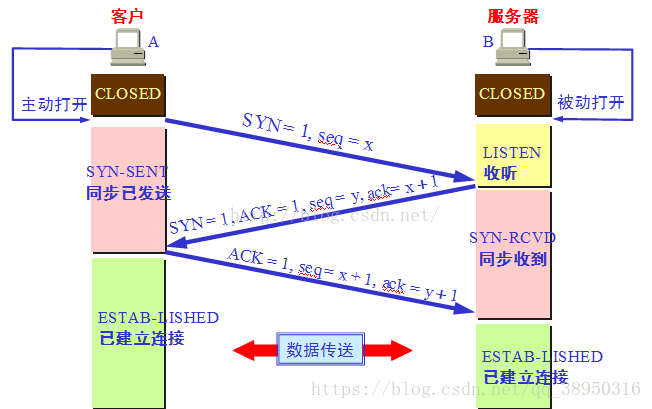
\includegraphics[height=1\linewidth,width=1\textwidth]{Figure/Three.png}
\caption{三次握手}
\end{figure}

1.第一次握手:Client将标志位SYN设置为1,随机产生一个值seq=J,并将数据包发送给Server,Client进入SYN\_SENT状态,等待Server确认。

2.第二次握手:Server收到数据包后由标志位SYN=1直到Client请求建立连接,Server将标志位SYN和ACK都设置为1,ack=J+1,随机产生一个值seq=K,并将该数据包发送给Client以确认连接请求,Server进入SYN\_RCVD状态。

3.第三次握手:Client收到确认后,检查Ack是否为J+1,ACK是否为1,如果正确则将标志位ACK置1,ACK=K+1,并将数该数据包发送给Server,Server检查ack是否为K+1,ACK是否为1,如果正确则连接建立成功,Client和Server进入ESTABLISHED状态,完成三次握手,随后Client和Server之间可以开始传输数据了。

总结:从这里介绍的可以看出,这里对SYN、ACK、ack、seq的输出都是有特点的,主要的特点就是,第一次握手和最后一次握手,都是只有两个变量,同时我们可以看出来,ACK=1是建立连接的必要条件,所以在第二次握手和第三次握手的时候,ACK=1都是城里的。对于ack,第二次和第第三次的特点是,第二次的ack是第一次产生的随机seq上加1,第三次ack是第二次随机产生的seq上加1。

\textbf{四次挥手}

四次挥手(Four-Way Wavehand)是断开TCP连接的过程,需要客户端和服务端总共发送4个包以确认连接的断开。在socket编程中,这一过程由客户端或服务端任一方执行close来出发,整个流程如图所示:




由于TCP连接是全双工的,因此,每个方向都必须要单独进行关闭,这一原则是当一方完成数据发送任务后,发送一个FIN来终止这一方向的连接,收到一个FIN只是意味这一方向上没有数据流动了,即不会再收到数据了,但是在这个TCP连接上仍然能够发送数据,直到这一方向也发送了FIN。首先进行关闭的一方将执行主动关闭,而另一方则执行被动关闭,上图描述的即使如此。

1.第一次挥手:Client发送一个FIN,用来关闭Client到Server的数据传送,Client进入FIN\_WAIT\_1状态。

2.第二次挥手:Server收到FIN后,发送一个ACK给Client,确认序号为收到序号+1(与SYN相同,一个FIN占用一个序号),Server进入CLOSE\_WAIT状态。

3.第三次挥手:Server发送一个FIN,用来关闭Server到Client的数据传送,Server进入LAST\_ACK状态。

4.第四次挥手:Client收到FIN后,Client进入TIME \_WAIT状态,接着发送一个ACK给Server,确认序号未收到序号+1,Server进入
CLOSED状态,完成四次挥手。


\textbf{Http和Https的区别}

1.https协议需要到ca申请证书,一般免费证书较少,因而需要一定费用。

2.http是超文本传输协议,信息是明文传输,https则是具有安全性的ssl加密传输协议。

3.http和https使用的是完全不同的连接方式,用的端口也不一样,前者是80,后者是443。

4.http的连接很简单,是无状态的;HTTPS协议是由SSL+HTTP协议构建的可进行加密传输、身份认证的网络协议,比http协议安全。

\textbf{TCP与UDP的区别}

1.TCP (Transmission Control Protocol)和UDP(User Datagram Protocol)协议属于传输层协议,它们之间的区别包括:

2.TCP是面向连接的,UDP是无连接的;

3.TCP是可靠的,UDP是不可靠的;

4.TCP只支持点对点通信,UDP支持一对一、一对多、多对一、多对多的通信模式;

5.TCP是面向字节流的,UDP是面向报文的;

6.TCP有拥塞控制机制;UDP没有拥塞控制,适合媒体通信;

7.TCP首部开销(20个字节)比UDP的首部开销(8个字节)要大;

\textbf{从输入网址到获得页面的过程}

浏览器查询 DNS,获取域名对应的IP地址:具体过程包括浏览器搜索自身的DNS缓存、搜索操作系统的DNS缓存、读取本地的Host文件和向本地DNS服务器进行查询等。对于向本地DNS服务器进行查询,如果要查询的域名包含在本地配置区域资源中,则返回解析结果给客户机,完成域名解析(此解析具有权威性);如果要查询的域名不由本地DNS服务器区域解析,但该服务器已缓存了此网址映射关系,则调用这个IP地址映射,完成域名解析(此解析不具有权威性)。如果本地域名服务器并未缓存该网址映射关系,那么将根据其设置发起递归查询或者迭代查询;

浏览器获得域名对应的IP地址以后,浏览器向服务器请求建立链接,发起三次握手;

TCP/IP链接建立起来后,浏览器向服务器发送HTTP请求;

服务器接收到这个请求,并根据路径参数映射到特定的请求处理器进行处理,并将处理结果及相应的视图返回给浏览器;

浏览器解析并渲染视图,若遇到对js文件、css文件及图片等静态资源的引用,则重复上述步骤并向服务器请求这些资源;

浏览器根据其请求到的资源、数据渲染页面,最终向用户呈现一个完整的页面。




\section{数据库}

数据库也是面试中常见的问题,对于数据库的面试,常见的问题是数据库设计的范式,数据库的查询优化,聚集索引和非聚集索引,MyISAM和InnoDB的区别,MySQL的binlog日志等,下面我们对涉及到的知识进行巩固。

\subsection{MyISAM和InnoDB}

1、MyISAM:默认表类型,它是基于传统的ISAM类型,ISAM是Indexed Sequential Access Method (有索引的顺序访问方法) 的缩写,它是存储记录和文件的标准方法。不是事务安全的,而且不支持外键,如果执行大量的select,insert MyISAM比较适合。

2、InnoDB:支持事务安全的引擎,支持外键、行锁、事务是他的最大特点。如果有大量的update和insert,建议使用InnoDB,特别是针对多个并发和QPS较高的情况。

\subsubsection{表锁差异}
MyISAM:

myisam只支持表级锁,用户在操作myisam表时,select,update,delete,insert语句都会给表自动加锁,如果加锁以后的表满足insert并发的情况下,可以在表的尾部插入新的数据。也可以通过lock table命令来锁表,这样操作主要是可以模仿事务,但是消耗非常大,
一般只在实验演示中使用。

InnoDB:

Innodb支持事务和行级锁,是innodb的最大特色。

事务的ACID属性:atomicity,consistent,isolation,durable。

并发事务带来的几个问题:更新丢失,脏读,不可重复读,幻读。

事务隔离级别:未提交读(Read uncommitted),已提交读(Read committed),可重复读(Repeatable read),可序列化(Serializable)

\begin{table}[]
    \caption{四种隔离级别的比较}
    \vspace{20pt}
    \centering
    \begin{tabular}{|l|c|c|c|c|}
        \hline
        读数据一致性及并发副作用、隔离级别&读数据一致性&脏读&不可重复读&幻读\\
        \hline
		为提交读(read uncommitted)&最低级别,不读物理上顺坏的数据&是&是&是\\
		已提交读(read committed)	&语句级&否&是&是\\
		可重复读(Repeatable red)	&事务级&否&否&是\\
		可序列化(Serializable)	&最高级别事务级&否&否&否\\
        \hline       
    \end{tabular}
    \label{bs02}
\end{table}

查看mysql的默认事务隔离级别“show global variables like ‘tx\_isolation’; ”

Innodb的行锁模式有以下几种:共享锁,排他锁,意向共享锁(表锁),意向排他锁(表锁),间隙锁。

注意:当语句没有使用索引,innodb不能确定操作的行,这个时候就使用的意向锁,也就是表锁

关于死锁:

什么是死锁?当两个事务都需要获得对方持有的排他锁才能完成事务,这样就导致了循环锁等待,也就是常见的死锁类型。

解决死锁的方法:

1、  数据库参数

2、  应用中尽量约定程序读取表的顺序一样

3、  应用中处理一个表时,尽量对处理的顺序排序

4、  调整事务隔离级别(避免两个事务同时操作一行不存在的数据,容易发生死锁)
\subsubsection{数据库文件差异}
MyISAM :

myisam属于堆表

myisam在磁盘存储上有三个文件,每个文件名以表名开头,扩展名指出文件类型。

.frm 用于存储表的定义

.MYD 用于存放数据

.MYI 用于存放表索引

myisam表还支持三种不同的存储格式:

静态表(默认,但是注意数据末尾不能有空格,会被去掉)

动态表

压缩表

InnoDB :

innodb属于索引组织表

innodb有两种存储方式,共享表空间存储和多表空间存储

两种存储方式的表结构和myisam一样,以表名开头,扩展名是.frm。

如果使用共享表空间,那么所有表的数据文件和索引文件都保存在一个表空间里,一个表空间可以有多个文件,通过innodb\_data\_file\_path和innodb\_data\_home\_dir参数设置共享表空间的位置和名字,一般共享表空间的名字叫ibdata1-n。

如果使用多表空间,那么每个表都有一个表空间文件用于存储每个表的数据和索引,文件名以表名开头,以.ibd为扩展名。

\subsubsection{索引差异}
1、关于自动增长

myisam引擎的自动增长列必须是索引,如果是组合索引,自动增长可以不是第一列,他可以根据前面几列进行排序后递增。

innodb引擎的自动增长咧必须是索引,如果是组合索引也必须是组合索引的第一列。

2、关于主键

myisam允许没有任何索引和主键的表存在,

myisam的索引都是保存行的地址。

innodb引擎如果没有设定主键或者非空唯一索引,就会自动生成一个6字节的主键(用户不可见)

innodb的数据是主索引的一部分,附加索引保存的是主索引的值。

3、关于count()函数

myisam保存有表的总行数,如果select count(*) from table;会直接取出出该值

innodb没有保存表的总行数,如果使用select count(*) from table;就会遍历整个表,消耗相当大,但是在加了wehre条件后,
myisam和innodb处理的方式都一样。

4、全文索引

myisam支持 FULLTEXT类型的全文索引

innodb不支持FULLTEXT类型的全文索引,但是innodb可以使用sphinx插件支持全文索引,并且效果更好。(sphinx   是一个开源软件,提供多种语言的API接口,可以优化mysql的各种查询)

5、delete from table

使用这条命令时,innodb不会从新建立表,而是一条一条的删除数据,在innodb上如果要清空保存有大量数据的表,最       好不要使用这个命令。(推荐使用truncate table,不过需要用户有drop此表的权限)

6、索引保存位置

myisam的索引以表名+.MYI文件分别保存。

innodb的索引和数据一起保存在表空间里。

\subsubsection{开发的注意事项}

1、可以用 show create table tablename 命令看表的引擎类型。

2、对不支持事务的表做start/commit操作没有任何效果,在执行commit前已经提交。

3、可以执行以下命令来切换非事务表到事务(数据不会丢失),innodb表比myisam表更安全:alter table tablename type=innodb;或者使用 alter table tablename engine = innodb;

4、默认innodb是开启自动提交的,如果你按照myisam的使用方法来编写代码页不会存在错误,只是性能会很低。如何在编写代码时候提高数据库性能呢?

a、尽量将多个语句绑到一个事务中,进行提交,避免多次提交导致的数据库开销。

b、在一个事务获得排他锁或者意向排他锁以后,如果后面还有需要处理的sql语句,在这两条或者多条sql语句之间程序应尽量少的进行逻辑运算和处理,减少锁的时间。

c、尽量避免死锁

d、sql语句如果有where子句一定要使用索引,尽量避免获取意向排他锁。

f、针对我们自己的数据库环境,日志系统是直插入,不修改的,所以我们使用混合引擎方式,ZION\_LOG\_DB照旧使用myisam存储引擎,只有ZION\_GAME\_DB,ZION\_LOGIN\_DB,DAUM\_BILLING使用Innodb引擎。

\subsubsection{究竟该怎么选择}

下面先让我们回答一些问题:   

◆你的数据库有外键吗?   

◆你需要事务支持吗?   

◆你需要全文索引吗?   

◆你经常使用什么样的查询模式?   

◆你的数据有多大?   
  
myisam只有索引缓存   
innodb不分索引文件数据文件 innodb buffer   
myisam只能管理索引,在索引数据大于分配的资源时,会由操作系统来cache;数据文件依赖于操作系统的cache。innodb不管是索引还是数据,都是自己来管理  
  
思考上面这些问题可以让你找到合适的方向,但那并不是绝对的。如果你需要事务处理或是外键,那么InnoDB 可能是比较好的方式。如果你需要全文索引,那么通常来说 MyISAM是好的选择,因为这是系统内建的,然而,我们其实并不会经常地去测试两百万行记录。所以,就算是慢一点,我们可以通过使用Sphinx从InnoDB中获得全文索引。  
  
数据的大小,是一个影响你选择什么样存储引擎的重要因素,大尺寸的数据集趋向于选择InnoDB方式,因为其支持事务处理和故障恢复。数据库的在小决定了故障恢复的时间长短,InnoDB可以利用事务日志进行数据恢复,这会比较快。而MyISAM可能会需要几个小时甚至几天来干这些事,InnoDB只需要几分钟。  
  
操作数据库表的习惯可能也会是一个对性能影响很大的因素。比如: COUNT() 在 MyISAM 表中会非常快,而在InnoDB 表下可能会很痛苦。而主键查询则在InnoDB下会相当相当的快,但需要小心的是如果我们的主键太长了也会导致性能问题。大批的inserts 语句在 MyISAM下会快一些,但是updates 在InnoDB下会更快一些——尤其在并发量大的时候。  
  
所以,到底你检使用哪一个呢?根据经验来看,如果是一些小型的应用或项目,那么MyISAM 也许会更适合。当然,在大型的环境下使用 MyISAM 也会有很大成功的时候,但却不总是这样的。如果你正在计划使用一个超大数据量的项目,而且需要事务处理或外键支持,那么你真的应该直接使用 InnoDB方式。但需要记住InnoDB 的表需要更多的内存和存储,转换100GB 的MyISAM 表到InnoDB 表可能会让你有非常坏的体验。  
  
对于支持事务的InnoDB类型的表,影响速度的主要原因是AUTOCOMMIT默认设置是打开的,而且程序没有显式调用BEGIN 开始事务,导致每插入一条都自动Commit,严重影响了速度。可以在执行sql前调用begin,多条sql形成一个事务(即使autocommit打开也可以),将大大提高性能。  

InnoDB

InnoDB 给 MySQL 提供了具有事务(commit)、回滚(rollback)和崩溃修复能力 (crash recovery capabilities)的事务安全(transaction-safe (ACID compliant))型表。 InnoDB 提供了行锁(locking on row level),提供与 Oracle 类型一致的不加锁读取(non- locking read in SELECTs)。这些特性均提高了多用户并发操作的性能表现。在InnoDB表中不需要扩大锁定 (lock escalation),因为 InnoDB 的列锁定(row level locks)适宜非常小的空间。 InnoDB 是 MySQL 上第一个提供外键约束(FOREIGN KEY constraints)的表引擎。  

InnoDB 的设计目标是处理大容量数据库系统,它的 CPU 利用率是其它基于磁盘的关系数据库引擎所不能比的。在技术上,InnoDB 是一套放在 MySQL 后台的完整数据库系统,InnoDB 在主内存中建立其专用的缓冲池用于高速缓冲数据和索引。 InnoDB 把数据和索引存放在表空间里,可能包含多个文件,这与其它的不一样,举例来说,在 MyISAM 中,表被存放在单独的文件中。InnoDB 表的大小只受限于操作系统的文件大小,一般为 2 GB。  
InnoDB所有的表都保存在同一个数据文件 ibdata1 中(也可能是多个文件,或者是独立的表空间文件),相对来说比较不好备份,免费的方案可以是拷贝数据文件、备份 binlog,或者用 mysqldump。  

MyISAM   

MyISAM 是MySQL缺省存贮引擎 .   
每张MyISAM 表被存放在三个文件 。frm 文件存放表格定义。 数据文件是MYD (MYData) 。 索引文件是 MYI (MYIndex) 引伸。   
因为MyISAM相对简单所以在效率上要优于InnoDB..小型应用使用MyISAM是不错的选择.   
MyISAM表是保存成文件的形式,在跨平台的数据转移中使用MyISAM存储会省去不少的麻烦   
  
以下是一些细节和具体实现的差别:   
  
1.InnoDB不支持FULLTEXT类型的索引。   
2.InnoDB 中不保存表的具体行数,也就是说,执行select count(*) from table时,InnoDB要扫描一遍整个表来计算有多少行,但是MyISAM只要简单的读出保存好的行数即可。注意的是,当count(*)语句包含 where条件时,两种表的操作是一样的。  
3.对于AUTO\_INCREMENT类型的字段,InnoDB中必须包含只有该字段的索引,但是在MyISAM表中,可以和其他字段一起建立联合索引。   
4.DELETE FROM table时,InnoDB不会重新建立表,而是一行一行的删除。   
5.LOAD TABLE FROM MASTER操作对InnoDB是不起作用的,解决方法是首先把InnoDB表改成MyISAM表,导入数据后再改成InnoDB表,但是对于使用的额外的InnoDB特性(例如外键)的表不适用。  

另外,InnoDB表的行锁也不是绝对的,如果在执行一个SQL语句时MySQL不能确定要扫描的范围,InnoDB表同样会锁全表,例如 update table set num=1 where name like “\%aaa\%”  

任何一种表都不是万能的,只用恰当的针对业务类型来选择合适的表类型,才能最大的发挥MySQL的性能优势。   

 
\subsubsection{重复地总结一遍}

1、MyISAM不支持事务,InnoDB是事务类型的存储引擎,当我们的表需要用到事务支持的时候,那肯定是不能选择MyISAM了。

2、MyISAM只支持表级锁,BDB支持页级锁和表级锁默认为页级锁,而InnoDB支持行级锁和表级锁默认为行级锁
 
表级锁:直接锁定整张表,在锁定期间,其他进程无法对该表进行写操作,如果设置的是写锁,那么其他进程读也不允许
 
MyISAM是表级锁定的存储引擎,它不会出现死锁问题
 
对于write,表锁定原理如下:
 
如果表上没有锁,在其上面放置一个写锁,否则,把锁定请求放在写锁队列中。
 
对于read,表锁定原理如下 :
 
如果表上没有写锁定,那么把一个读锁放在其上面,否则把锁请求放在读锁定队列中
 
当一个锁定被释放时,表可被写锁定队列中的线程得到,然后才是读锁定队列中的线程。这意味着,如果你在一个表上有许多更新,那么你的SELECT语句将等到所有的写锁定线程执行完。

行级锁:只对指定的行进行锁定,其他进程还是可以对表中的其他行进行操作的。
 
行级锁是Mysql粒度最小的一种锁,它能大大的减少数据库操作的冲突,但是粒度越小实现成本也越大。
 
行级锁可能会导致“死锁”,那到底是怎么导致的呢,分析原因:Mysql行级锁并不是直接锁记录,而是锁索引。索引分为主键索引和非主键索引两种,如果一条sql语句操作了主键索引,那么Mysql就会锁定这个主键索引,如果sql语句操作的是非主键索引,那么Mysql会先锁定这个非主键索引,再去锁定主键索引。
 
在UPDATE 和 DELETE操作时Mysql不仅会锁定所有WHERE 条件扫描过得索引,还会锁定相邻的键值。
 
“死锁”举例分析:
 
表Test:(ID,STATE,TIME)  主键索引:ID  非主键索引:STATE
 
当执行"UPDATE  STATE =1011 WHERE STATE=1000"  语句的时候会锁定STATE索引,由于STATE 是非主键索引,所以Mysql还会去请求锁定ID索引
 
当另一个SQL语句与语句1几乎同时执行时:“UPDATE STATE=1010 WHERE ID=1”  对于语句2 Mysql会先锁定ID索引,由于语句2操作了STATE字段,所以Mysql还会请求锁定STATE索引。这时。彼此锁定着对方需要的索引,又都在等待对方释放锁定。所以出现了"死锁"的情况。
 
行级锁的优点:
 
有许多线程访问不同的行时,只存在少量的冲突。
 
回滚时只有少量的更改
 
可以长时间锁定单一的行
 
行级锁缺点:
 
相对于页级锁和表级锁来说占用了更多的内存
 
当表的大部分行在使用时,比页级锁和表级锁慢,因为你必须获得更多的锁
 
当在大部分数据上经常使用GROUP BY操作,肯定会比表级锁和页级锁慢。
 
页级锁:表级锁速度快,但是冲突多;行级锁速度慢,但冲突少;页级锁就是他俩折中的,一次锁定相邻的一组记录。

3、MyISAM引擎不支持外键,InnoDB支持外键

4、MyISAM引擎的表在大量高并发的读写下会经常出现表损坏的情况
 
我们以前做的项目就遇到这个问题,表的INSERT 和 UPDATE操作很频繁,原来用的MyISAM引擎,导致表隔三差五就损坏,后来更换成了InnoDB引擎。
 
其他容易导致表损坏原因:
 
服务器突然断电导致数据文件损坏,强制关机(mysqld未关闭情况下)导致表损坏
 
mysqld进程在写入操作的时候被杀掉
 
磁盘故障
 
表损坏常见症状:
 
查询表不能返回数据或返回部分数据
 
打开表失败: Can’t open file: ‘×××.MYI’ (errno: 145) 。
 
Error: Table 'p' is marked as crashed and should be repaired 。

Incorrect key file for table: '...'. Try to repair it
 
Mysql表的恢复:

对于MyISAM表的恢复:

可以使用Mysql自带的myisamchk工具: myisamchk -r tablename  或者 myisamchk -o tablename(比前面的更保险) 对表进行修复

5、对于count()查询来说MyISAM更有优势

因为MyISAM存储了表中的行数记录,执行SELECT COUNT() 的时候可以直接获取到结果,而InnoDB需要扫描全部数据后得到结果。

但是注意一点:对于带有WHERE 条件的 SELECT COUNT()语句两种引擎的表执行过程是一样的,都需要扫描全部数据后得到结果

6、 InnoDB是为处理巨大数据量时的最大性能设计,它的CPU效率可能是任何其它基于磁盘的关系数据库引擎所不能匹敌的。

7、MyISAM支持全文索引(FULLTEXT),InnoDB不支持

8、MyISAM引擎的表的查询、更新、插入的效率要比InnoDB高

网上截取了前辈们测试结论: 

测试方法:连续提交10个query, 表记录总数:38万 , 时间单位 s
\begin{table}[]
    \caption{四种隔离级别的比较}
    \vspace{20pt}
    \centering
    \begin{tabular}{|l||c|c|c|}
        \hline
        引擎类型 &MyISAM&InnoDB&性能相差\\
        \hline
        引擎类型             &      MyISAM           &     InnoDB      &        性能相差\\
        count               &      0.0008357     &       3.0163      &          3609\\
        查询主键             &   0.005708         &     0.1574        &        27.57\\
        查询非主键           &    24.01         &         80.37      &          3.348\\
        更新主键             &  0.008124         &      0.8183        &        100.7\\
        更新非主键           &   0.004141       &     0.02625        &      6.338\\
        插入                 &    0.004188      &      0.3694       &         88.21\\
        \hline       
    \end{tabular}
    \label{bs3}
\end{table}
(1)加了索引以后,对于MyISAM查询可以加快:4 206.09733倍,对InnoDB查询加快510.72921倍,同时对MyISAM更新速度减慢为原来的1/2,InnoDB的更
  新速度减慢为原来的1/30。要看情况决定是否要加索引,比如不查询的log表,不要做任何的索引。
 
 (2)如果你的数据量是百万级别的,并且没有任何的事务处理,那么用MyISAM是性能最好的选择。
 
 (3)InnoDB表的大小更加的大,用MyISAM可省很多的硬盘空间。
        在我们测试的这个38w的表中,表占用空间的情况如下:
   \begin{table}[]
    \caption{38w的表所占空间}
    \vspace{20pt}
    \centering
    \begin{tabular}{|l|c|c|c|}
        \hline
            引擎类型       &             MyISAM     &        InnoDB\\
            数据            &          53,924 KB      &    58,976 KB\\
            索引             &         13,640 KB     &     21,072 KB\\
            占用总空间      &        67,564 KB       &   80,048 KB\\
          \hline       
    \end{tabular}
    \label{bs4}
\end{table}

另外一个176W万记录的表, 表占用空间的情况如下:
\begin{table}[]
\caption{176W万记录的表所占空间}
\vspace{20pt}
\centering
\begin{tabular}{|l|c|c|c|}
\hline
引擎类型        &        MyIsam &             InnorDB\\
数据           &       56,166 KB    &      90,736 KB\\
索引           &       67,103 KB   &       88,848 KB\\
占用总空间      &  123,269 KB     &   179,584 KB\\
 \hline       
 \end{tabular}
 \label{bs5}
\end{table}
\subsubsection{性能对比}
测试的版本是mysql  Ver 14.14 Distrib 5.1.49, for debian-linux-gnu (i686),使用的是Innodb plugin 1.0.8(官方称比built-in版本性能更好)和默认的MyISAM。

测试机器是笔记本,配置如下:Intel 酷睿2双核 P8600,2G*2 DDR3 1066内存,320G硬盘5400转。

测试一:数据插入性能测试,这里我分别对innodb\_flush\_log\_at\_trx\_commit参数打开和关闭都测了了一下,每次测试都是运行40s,表中数字都是实际插入条数。
\begin{table}[]
\caption{数据插入性能测试}
\vspace{20pt}
\centering
\begin{tabular}{|l|c|c|c|}
\hline
特点           &   MyISAM           &      Innodb (打开)  &    Innodb (关闭)\\

单线程,逐个插入     &    120000    &             60000         &     60000\\

4线程,逐个插入      &    40000*4    &            20000*4       &     40000*4\\

单线程,批量100条/次插入&  3600*100   &            800*100      &      3000*100\\

单线程,批量200条/次插入 & 1800*200    &           400*200      &      1600*200\\
\hline       
\end{tabular}
\label{bs5}
\end{table}

可以发现批量插入的性能远高于单条插入,但是一次批量的大小对性能影响不大。每条记录是否都刷新日志的参数对innodb性能的影响巨大。总体上来说,MyISAM性能更优一点。这里有一点需要注意,在插入测试过程中,我对系统资源进行了监控,发现MyISAM对系统资源占用很低,但是Innodb对磁盘占用却很高,应该是对事务控制多了很多需要记录的日志。

测试二:数据读取性能测试。每次随机读取1000条记录,反复进行读取。
\begin{table}[]
\caption{数据读取性能测试}
\vspace{20pt}
\centering
\begin{tabular}{c|c|c|}
\hline
特点     &   MyISAM     &   Innodb\\
单线程,200次读取      &   5.7s  &16.7s\\
4线程,200次读取       &   12s& 40.8s\\
\hline       
\end{tabular}
\label{bs5}
\end{table}
可以看出MyISAM的读取性能非常恐怖,性能差距在3倍的样子。

以上两个测试发现MyISAM在无事务的需求下几乎完胜,但是要知道它是表锁,Innodb是行锁,那么在并发读写同时存在的情况下,那结果会是怎么样呢?!

测试三:两个线程并发写入,2个线程并发读取。
\begin{table}[]
\caption{两个线程并发写入}
\vspace{20pt}
\centering
\begin{tabular}{c|c|c|}
\hline
特点    &  MyISAM                      &           Innodb\\
逐个插入              &  写入40s:10000*2 读取200次*2:14s     &   写入40s:60000*2 读取200次*2:50s\\
批量100条/次插入      &  写入40s:1000*100*2 读取200次*2:10s   &   写入40s:1500*100*2 读取200次*2:50s\\
\hline       
\end{tabular}
\label{bs5}
\end{table}

这下立刻显示出Innodb在并发情况下强劲的性能,几乎没有什么性能衰减。而MyISAM单条插入速度变得非常慢,批量插入也下降了40\%性能。

总结一下,在写多读少的应用中还是Innodb插入性能更稳定,在并发情况下也能基本,如果是对读取速度要求比较快的应用还是选MyISAM。
\subsection{聚集索引与非聚集索引的总结}
\subsubsection{索引简介}
众所周知,索引是关系型数据库中给数据库表中一列或多列的值排序后的存储结构,SQL的主流索引结构有B+树以及Hash结构,聚集索引以及非聚集索引用的是B+树索引。这篇文章会总结SQL Server以及MySQL的InnoDB和MyISAM两种 SQL的索引。
SQL Sever索引类型有:唯一索引,主键索引,聚集索引,非聚集索引。
MySQL 索引类型有:唯一索引,主键(聚集)索引,非聚集索引,全文索引。
\subsubsection{聚集索引}
聚集(clustered)索引,也叫聚簇索引。
定义:数据行的物理顺序与列值(一般是主键的那一列)的逻辑顺序相同,一个表中只能拥有一个聚集索引。
单单从定义来看是不是显得有点抽象,打个比方,一个表就像是我们以前用的新华字典,聚集索引就像是拼音目录,而每个字存放的页码就是我们的数据物理地址,我们如果要查询一个“哇”字,我们只需要查询“哇”字对应在新华字典拼音目录对应的页码,就可以查询到对应的“哇”字所在的位置,而拼音目录对应的A-Z的字顺序,和新华字典实际存储的字的顺序A-Z也是一样的,如果我们中文新出了一个字,拼音开头第一个是B,那么他插入的时候也要按照拼音目录顺序插入到A字的后面,现在用一个简单的示意图来大概说明一下在数据库中的样子:
\begin{table}[]
    \caption{数据库样例}
    \vspace{20pt}
    \centering
    \begin{tabular}{p{2cm}p{3cm}p{2.5cm}p{2.5cm}}
        \hline
        地址 & id  & username & score\\
        \hline
        0x01&	1	&小明	&90\\
		0x02	&2	&小红&	80\\
		0x03&	3	&小华&	92\\
		..	&..	&..	&..\\
		0xff&	256	&小英&	70\\
        \hline       
    \end{tabular}
    \label{bs2}
\end{table}
注:第一列的地址表示该行数据在磁盘中的物理地址,后面三列才是我们SQL里面用的表里的列,其中id是主键,建立了聚集索引。
结合上面的表格就可以理解这句话了吧:数据行的物理顺序与列值的顺序相同,如果我们查询id比较靠后的数据,那么这行数据的地址在磁盘中的物理地址也会比较靠后。而且由于物理排列方式与聚集索引的顺序相同,所以也就只能建立一个聚集索引了。
\begin{figure}[htbp]
\centering
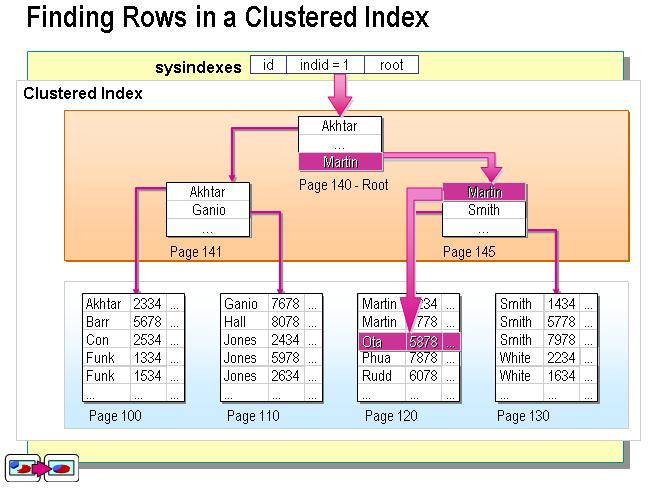
\includegraphics[height=1\linewidth,width=1\textwidth]{Figure/index0.png}
\caption{聚集索引实际存放的示意图}
\end{figure}
从上图可以看出聚集索引的好处了,索引的叶子节点就是对应的数据节点(MySQL的MyISAM除外,此存储引擎的聚集索引和非聚集索引只多了个唯一约束,其他没什么区别),可以直接获取到对应的全部列的数据,而非聚集索引在索引没有覆盖到对应的列的时候需要进行二次查询,后面会详细讲。因此在查询方面,聚集索引的速度往往会更占优势。

创建聚集索引

如果不创建索引,系统会自动创建一个隐含列作为表的聚集索引。

1.创建表的时候指定主键(注意:SQL Sever默认主键为聚集索引,也可以指定为非聚集索引,而MySQL里主键就是聚集索引)
create table t1(
    id int primary key,
    name nvarchar(255)
)
2.创建表后添加聚集索引

SQL Server

create clustered index clustered\_index on table\_name(colum\_name)

MySQL

alter table table\_name add primary key(colum\_name)

值得注意的是,最好还是在创建表的时候添加聚集索引,由于聚集索引的物理顺序上的特殊性,因此如果再在上面创建索引的时候会根据索引列的排序移动全部数据行上面的顺序,会非常地耗费时间以及性能。

\subsubsection{非聚集索引}

\textbf{非聚集(unclustered)索引}

定义:该索引中索引的逻辑顺序与磁盘上行的物理存储顺序不同,一个表中可以拥有多个非聚集索引。

其实按照定义,除了聚集索引以外的索引都是非聚集索引,只是人们想细分一下非聚集索引,分成普通索引,唯一索引,全文索引。如果非要把非聚集索引类比成现实生活中的东西,那么非聚集索引就像新华字典的偏旁字典,他结构顺序与实际存放顺序不一定一致。

\begin{figure}[htbp]
\centering
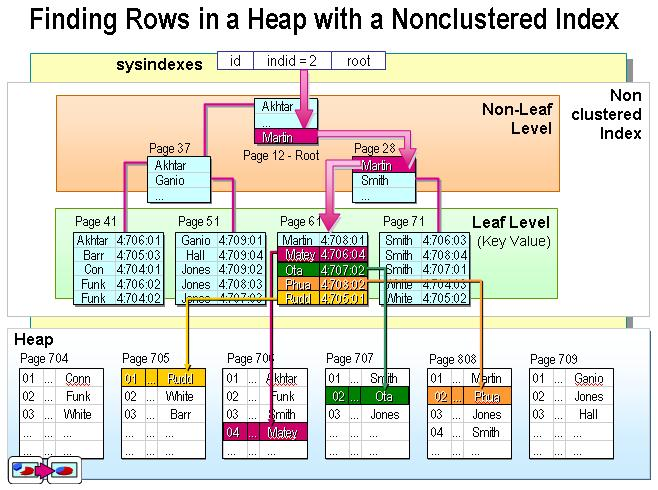
\includegraphics[height=1\linewidth,width=1\textwidth]{Figure/index1.png}
\caption{非聚集索引实际存放的示意图}
\end{figure}
非聚集索引的二次查询问题
非聚集索引叶节点仍然是索引节点,只是有一个指针指向对应的数据块,此如果使用非聚集索引查询,而查询列中包含了其他该索引没有覆盖的列,那么他还要进行第二次的查询,查询节点上对应的数据行的数据。
如有以下表t1:
\begin{table}[]
    \caption{数据库样例}
    \vspace{20pt}
    \centering
    \begin{tabular}{p{3cm}p{2.5cm}p{2.5cm}}
        \hline
        id  & username & score\\
        \hline
        1	&小明	&90\\
		2	&小红&	80\\
		3	&小华&	92\\
		..	&..	&..\\
		256	&小英&	70\\
        \hline       
    \end{tabular}
    \label{bs2}
\end{table}

以及聚集索引clustered index(id), 非聚集索引index(username)。
使用以下语句进行查询,不需要进行二次查询,直接就可以从非聚集索引的节点里面就可以获取到查询列的数据。

select id, username from t1 where username = '小明'
select username from t1 where username = '小明'
但是使用以下语句进行查询,就需要二次的查询去获取原数据行的score:

select username, score from t1 where username = '小明'
在SQL Server里面查询效率如下所示,Index Seek就是索引所花费的时间,Key Lookup就是二次查询所花费的时间。可以看的出二次查询所花费的查询开销占比很大,达到50\%。
\begin{figure}[htbp]
\centering
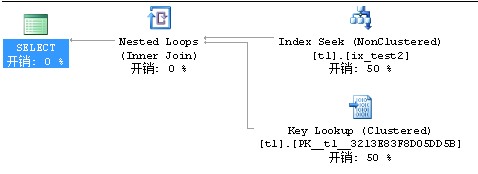
\includegraphics[height=0.2\linewidth,width=0.5\textwidth]{Figure/index2.png}
\caption{非聚集索引实际存放的示意图}
\end{figure}

在SQL Server里面会对查询自动优化,选择适合的索引,因此如果在数据量不大的情况下,SQL Server很有可能不会使用非聚集索引进行查询,而是使用聚集索引进行查询,即便需要扫描整个聚集索引,效率也比使用非聚集索引效率要高。
\begin{figure}[htbp]
\centering
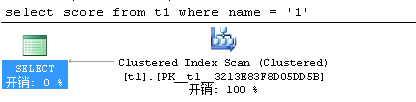
\includegraphics[height=0.2\linewidth,width=0.5\textwidth]{Figure/index3.png}
\caption{非聚集索引实际存放的示意图}
\end{figure}
本人试过在含有30w行表上建立非聚集索引,查询非聚集索引覆盖以外的列就会变成聚集索引的全索引扫描(index scan)查询来避免二次查询,而在另外一张200w行表才会用到非聚集索引seek对应的列再进行kek lookup,有关于SQL Server的有Index seek,index scan, table scan,key LookUp这几个概念,可以查看这个blog,描写比较详细。
但在MySQL里面就算表里数据量少且查询了非键列,也不会使用聚集索引去全索引扫描,但如果强制使用聚集索引去查询,性能反而比非聚集索引查询要差,这就是两种SQL的不同之处。
还有一点要注意的是非聚集索引其实叶子节点除了会存储索引覆盖列的数据,也会存放聚集索引所覆盖的列数据。
如何解决非聚集索引的二次查询问题
复合索引(覆盖索引)
建立两列以上的索引,即可查询复合索引里的列的数据而不需要进行回表二次查询,如index(col1, col2),执行下面的语句
select col1, col2 from t1 where col1 = '213';
要注意使用复合索引需要满足最左侧索引的原则,也就是查询的时候如果where条件里面没有最左边的一到多列,索引就不会起作用。
在SQL Server中还有include的用法,可以把非聚集索引里包含的列包含进来,而不一定需要建立复合索引。
\subsubsection{总结与使用心得}
使用聚集索引的查询效率要比非聚集索引的效率要高,但是如果需要频繁去改变聚集索引的值,写入性能并不高,因为需要移动对应数据的物理位置。
非聚集索引在查询的时候可以的话就避免二次查询,这样性能会大幅提升。
不是所有的表都适合建立索引,只有数据量大表才适合建立索引,且建立在选择性高的列上面性能会更好。
在这部分我们进行开发的时候,测试用例是需要进行分析的。首先就是功能测试,然后是边界值测试,再就是特殊输入测试。这三个都满足的时候才能进行最后的分析。


\subsection{MySQL的binlog}


\subsection{刷题}
在研究生进行找工作的时候,我们应该有一个比较好的安排,主要的工作是实习,论文,比赛,项目这几个部分,现在已经知道的是,比赛参加的是数学建模,论文没有,但是有一篇专利勉强能达到毕业要求,项目有个小的项目,实习看起来是不可能的了。后面有时间的话,需要专注于刷leetcode和牛客。多多看算算法和程序设计、计算机网络等相关知识,进针对性的复习。然后对毕业的大论文和小论文进行一番的思路等方法的分析。



\bibliographystyle{plain}
\bibliography{ref}
\end{document}